\documentclass{template/openetcs_article}
% Use the option "nocc" if the document is not licensed under Creative Commons
% \documentclass[nocc]{template/openetcs_article}
\usepackage{lipsum,url}
\usepackage{xspace}
\usepackage{graphicx}
\usepackage{fixme}
\usepackage{lscape} 
\usepackage{pgfgantt}
\usepackage{adjustbox}
\usepackage{datetime}
\usepackage{url}
\usepackage{amsmath}
\usepackage{algorithm}
\usepackage{hyperref}
\usepackage{tikz}
\usetikzlibrary{arrows,automata}
\usepackage{hyperref}
\usepackage{booktabs}
\usepackage{enumerate}
\graphicspath{{schema/}}
\usepackage{amsfonts}
\definecolor{hblue}{RGB}{79,129,189}

% user specified macros


\newcommand{\VV}{Verification \& Validation\xspace}
\newcommand{\vv}{verification \& validation\xspace}

\def\CC{{C\nolinebreak[4]\hspace{-.05em}\raisebox{.4ex}{\tiny\bf ++}}}

\newcommand{\bitwalker}{\mbox{\texttt{Bitwalker}}\xspace}

\newcommand{\poke}{\mbox{\texttt{Bitwalker\_Poke}}\xspace}
\newcommand{\peek}{\mbox{\texttt{Bitwalker\_Peek}}\xspace}
\newcommand{\acsl}{\mbox{\textsf{ACSL}}\xspace}
\newcommand{\isoc}{\mbox{\textsf{C}}\xspace}
\newcommand{\framac}{\mbox{\textsf{Frama-C}}\xspace}
\newcommand{\framacwp}{\mbox{\textsf{Frama-C\slash WP}}\xspace}
\newcommand{\why}{\mbox{\textsf{Why}}\xspace}
\newcommand{\wpframac}{\mbox{\textsf{WP}}\xspace}
\newcommand{\altergo}{\mbox{\textsf{Alt-Ergo}}\xspace}
\newcommand{\qed}{\mbox{\textsf{Qed}}\xspace}
\newcommand{\cvc}{\mbox{\textsf{CVC4}}\xspace}
\newcommand{\z}{\mbox{\textsf{Z3}}\xspace}
\newcommand{\coq}{\mbox{\textsf{Coq}}\xspace}
\newcommand{\cealist}{\mbox{\textsf{CEA LIST}}\xspace}

\newcommand{\inl}[1]{\lstinline[style=inline]{#1}}




\graphicspath{{./template/}{.}{./images/}}
\begin{document}
\frontmatter
\project{openETCS}

% Please do not change anything above this line ============================ The
% document metadata is defined below

\reportnum{OETCS/WP4/D4.2.1}

% define your workpackage or task here
\wp{openETCS@ITEA Work Package 4.2: ``Verification \& Validation of the Formal Model''}

% set a title here
\title{D.4.2.1 1st interim V\&V report on the applicability of the V\&V approach to the formal abstract model}

% set a subtitle here
\subtitle{}

% set the date of the report here
\date{January 2014}

% define a list of authors and their affiliation here
\author{Ana Cavalli \and João Santos \and Huu-Nghia Nguyen}

\affiliation{Institut Mines-Télécom}

\author{Marc~Behrens}

\affiliation{Deutsches Zentrum für Luft und Raumfahrt e.V.}

  
\author{Stefan Rieger}

\affiliation{TWT GmbH Science \& Inovation}

\author{Cécile Braunstein}
\affiliation{Uni Bremen}
  
\author{Uwe Steinke}
\affiliation{Siemens}

\author{Benoît~Lucet \and Matthias Güdemann \and Brice~Gombault \and Marielle~Petit-Doche} 

\affiliation{Systerel}

\author{Alexander Nitsch \& Benjamin Beichler}

\affiliation{University of Rostock}
 
\author{Silvano Dal Zilio \and Ning Ge}

\affiliation{LAAS-CNRS}

\author{Marc Pantel} 
  
\affiliation{INPT}
 
% define the coverart
\coverart[width=350pt]{openETCS_EUPL}

% define the type of report
\reporttype{}



% \begin{abstract} define an abstract here

% \lipsum[12-13]

% \end{abstract}

% ============================= Do not change the next three lines
\maketitle \tableofcontents \listoffiguresandtables \newpage
% =============================

% The actual document starts below this line =============================


% Start here

\section{Introduction}
This verification evaluated in five different approaches that the design conforms to an excerpt of Subset-026 \cite{unisig_subset-026_2012}  related to the specification \cite{tsi-2012-88-eu} \cite{tsi-2012-696-eu}.  It is the first of three reports. It is performed before a design or development process is available. The design used for verification in this report is created and adapted to improve later results of verificatoin. Due to the applicable restrictions the results of the first report focus on the verificatoin itself rather than to give a verdict about conformity of design. All following reports will focus solely on the design provided by the work package "Modelling – Code Generation".

To ensure the correctness and consistency of a design model and its implementation, the
validation and verification has to be performed alongside with the modeling process. 
As the model and code of the EVC are produced by WP3,
thus this task will be performed repeatedly during WP3 and will provide
feedback to it.

This document presents the interim results of the first iteration of
verification and validation of formal model.
Since the actual formal model of the ETCS system, provided by WP3, has not
yet been initiated, no ``real'' input is currently applied.

% This deliverable presents interim results from different partners from the
% project.
The following sections present the contributions of the partners: 
\begin{itemize}
  \item Institut Mines-Télécom: Verification of the Movement Authority (Subset-026~\cite{unisig_subset-026_2012} chapter 3.8)
  \item TWT GmbH Science \& Innovation: Verification of Procedures (Subset-026 chapter 5)
  \item University of Bremen: Verification of the Management of the Radio
  Comumunication (Subset-026 chapter 3.5)
  \item University of Rostock: Verification of the Speed and distance  Monitoring  (Subset-026 chapter 3.13)
  \item Systerel: Verification of Procedure on-Sight (Subset-026 chapter 5) and the Management of Radio Communication (Subset-026 chapter 3.5)
  \item LAAS and INPT: Verification of the Speed and Distance Monitoring (Subset-026 chapter 3.13)
\end{itemize}

\newpage
\section{Institut Mines-Télécom: Verification of the Movement Authority}

\subsection{Introduction}

We focus on applying model-based formal methods on validation and verification
(V\&V) of the ETCS system.
An overview of our approach is depicted in Figure~\ref{fig:approach}.

\begin{figure}[!htbp]
\begin{center}
  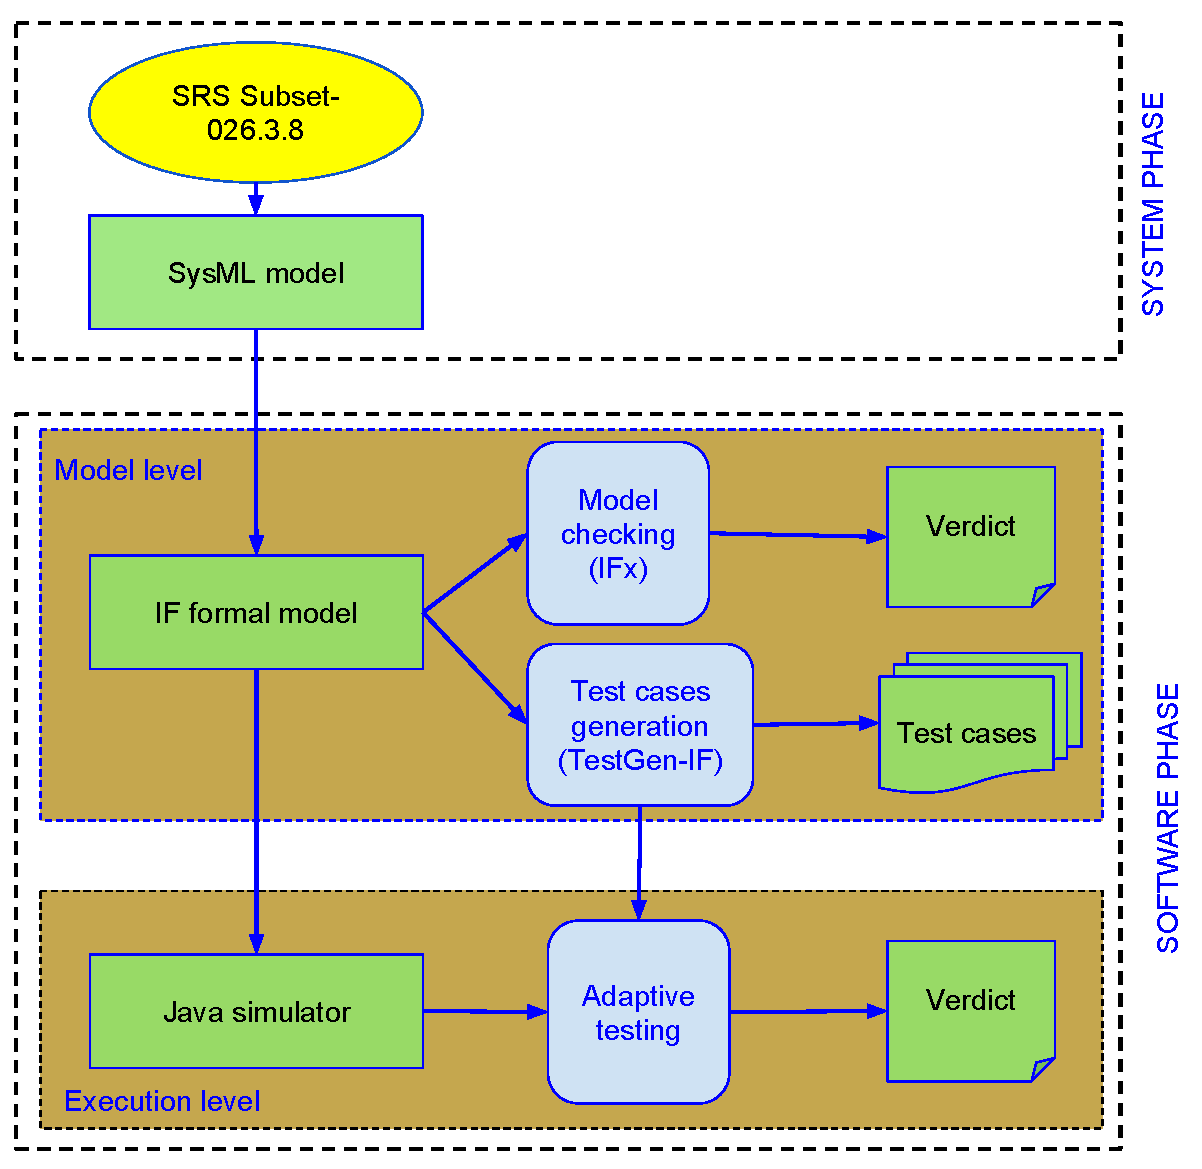
\includegraphics[width=.7\textwidth]{figures/TSP-approach.pdf}
  \caption{Overview of Institut Telecom-Mines' Approach}
  \label{fig:approach}
\end{center}
\end{figure}


In the openETCS project, the system requirement specifications are represented
by using SysML models. We validate and verify the models on two aspects,
model-level and execution-level, by using two model-based techniques:
model-checking and model-based testing.
At the model-level, V\&V is done through model-checking, by using IFx tool, of
IF formal models which are representations of the SysML models.
As model-checking techniques check exhaustively models, hence it may be
expensive in some special cases where we intend to check some properties of
models in some explicit conditions.
In such a case, model-based testing is a low-cost alternative.
At the execution-level, we encode the SysML models by Java simulators that are
then used to execute some tests.
We also illustrate the consistency of two aspects by applying test cases, that
are generated by TestGen-IF tool at the model-level, on our Java simulators,
i.e., all tests must give {\em pass} verdict

The automatic translations from SysML models to IF models to Java simulators are
being studied. Furthermore, as the actual models provided by WP3 have not yet
been initiated, we started with a formal model that is a finite state machine
augmented with continuous variables and guards. This model can be considered as
an abstract version of ETCS model and it can be refined in our future steps,
e.g., the MOVE function mode of the TRAIN can be refined to SHUNTING,
TRIP function modes of OBU in Subset-026.4.4.

%%%%%%%%%%%%%%%%%%%%%%%%%%%%%%%%%%%%%%%%%%%%%%%%%%%%%%%%%%%%%%%%%%%%%%%%%%%%%%
\subsection{Verification on IF model}
\subsubsection{Object of Verification}
The object of verification is an IF model representing the Movement Authority of
the train.

\subsubsection{Available Specification}
The Movement Authority is described in Subset-026, chapter 3.8. This chapter
gives (1) the definitions and structure of the movement authority, 
(2) the procedures of OBU to send a Movement Authority request to
the RBC and to receive a Movement Authority response from the RBC;
and (3) the use of Movement Authority on the OBU.

%Chapter 4.4 of Subset-026 describes in detail 16 different movement modes of
% OBU such as ISOLATION, TRIP, STAND BY, \ldots. At the moment, we generalize these modes onto
%two abstract modes: MOVE and STOP specifying when the train are moving or not.

\subsubsection{Detailed Verification Plan}

\paragraph{Goal} 
We intend firstly to model the Movement Authority of OBU described in
Subset-026-3.8. We then use the model to validate the safety
properties and to generate the test.




\paragraph{Method/Approach}


\paragraph{Means}

We consider an ETFSM (Extended Timed Finite State Machine) as a formal model
from which test cases for verifying the safety aspects of the developed
implementations can be automatically generated.
Formally, 
    an ETFSM is a tuple 
    $(S, s_0, E, T,  \Delta, v_0)$ where:
    $S$ is a non-empty finite set of states with $s_0 \in S$ as the
        initial state,
 $E$ is a finite set of events,
 $T$ is a set of transitions, 
 $\Delta \subset S \to S \times (\mathbb{N} \cup \{ \infty \})$ is timeout function, and
 $\vec{v}_0$ is the vector of initial values of the context variables.
The timeout function $\Delta$ limits an interval by which a trigger of
transition must occur (thus the transition will be fired). 
When the interval ends, the transition will be automatically fired in spite of
its trigger has not yet occurred.


\begin{figure}[!htbp]
\begin{center}
  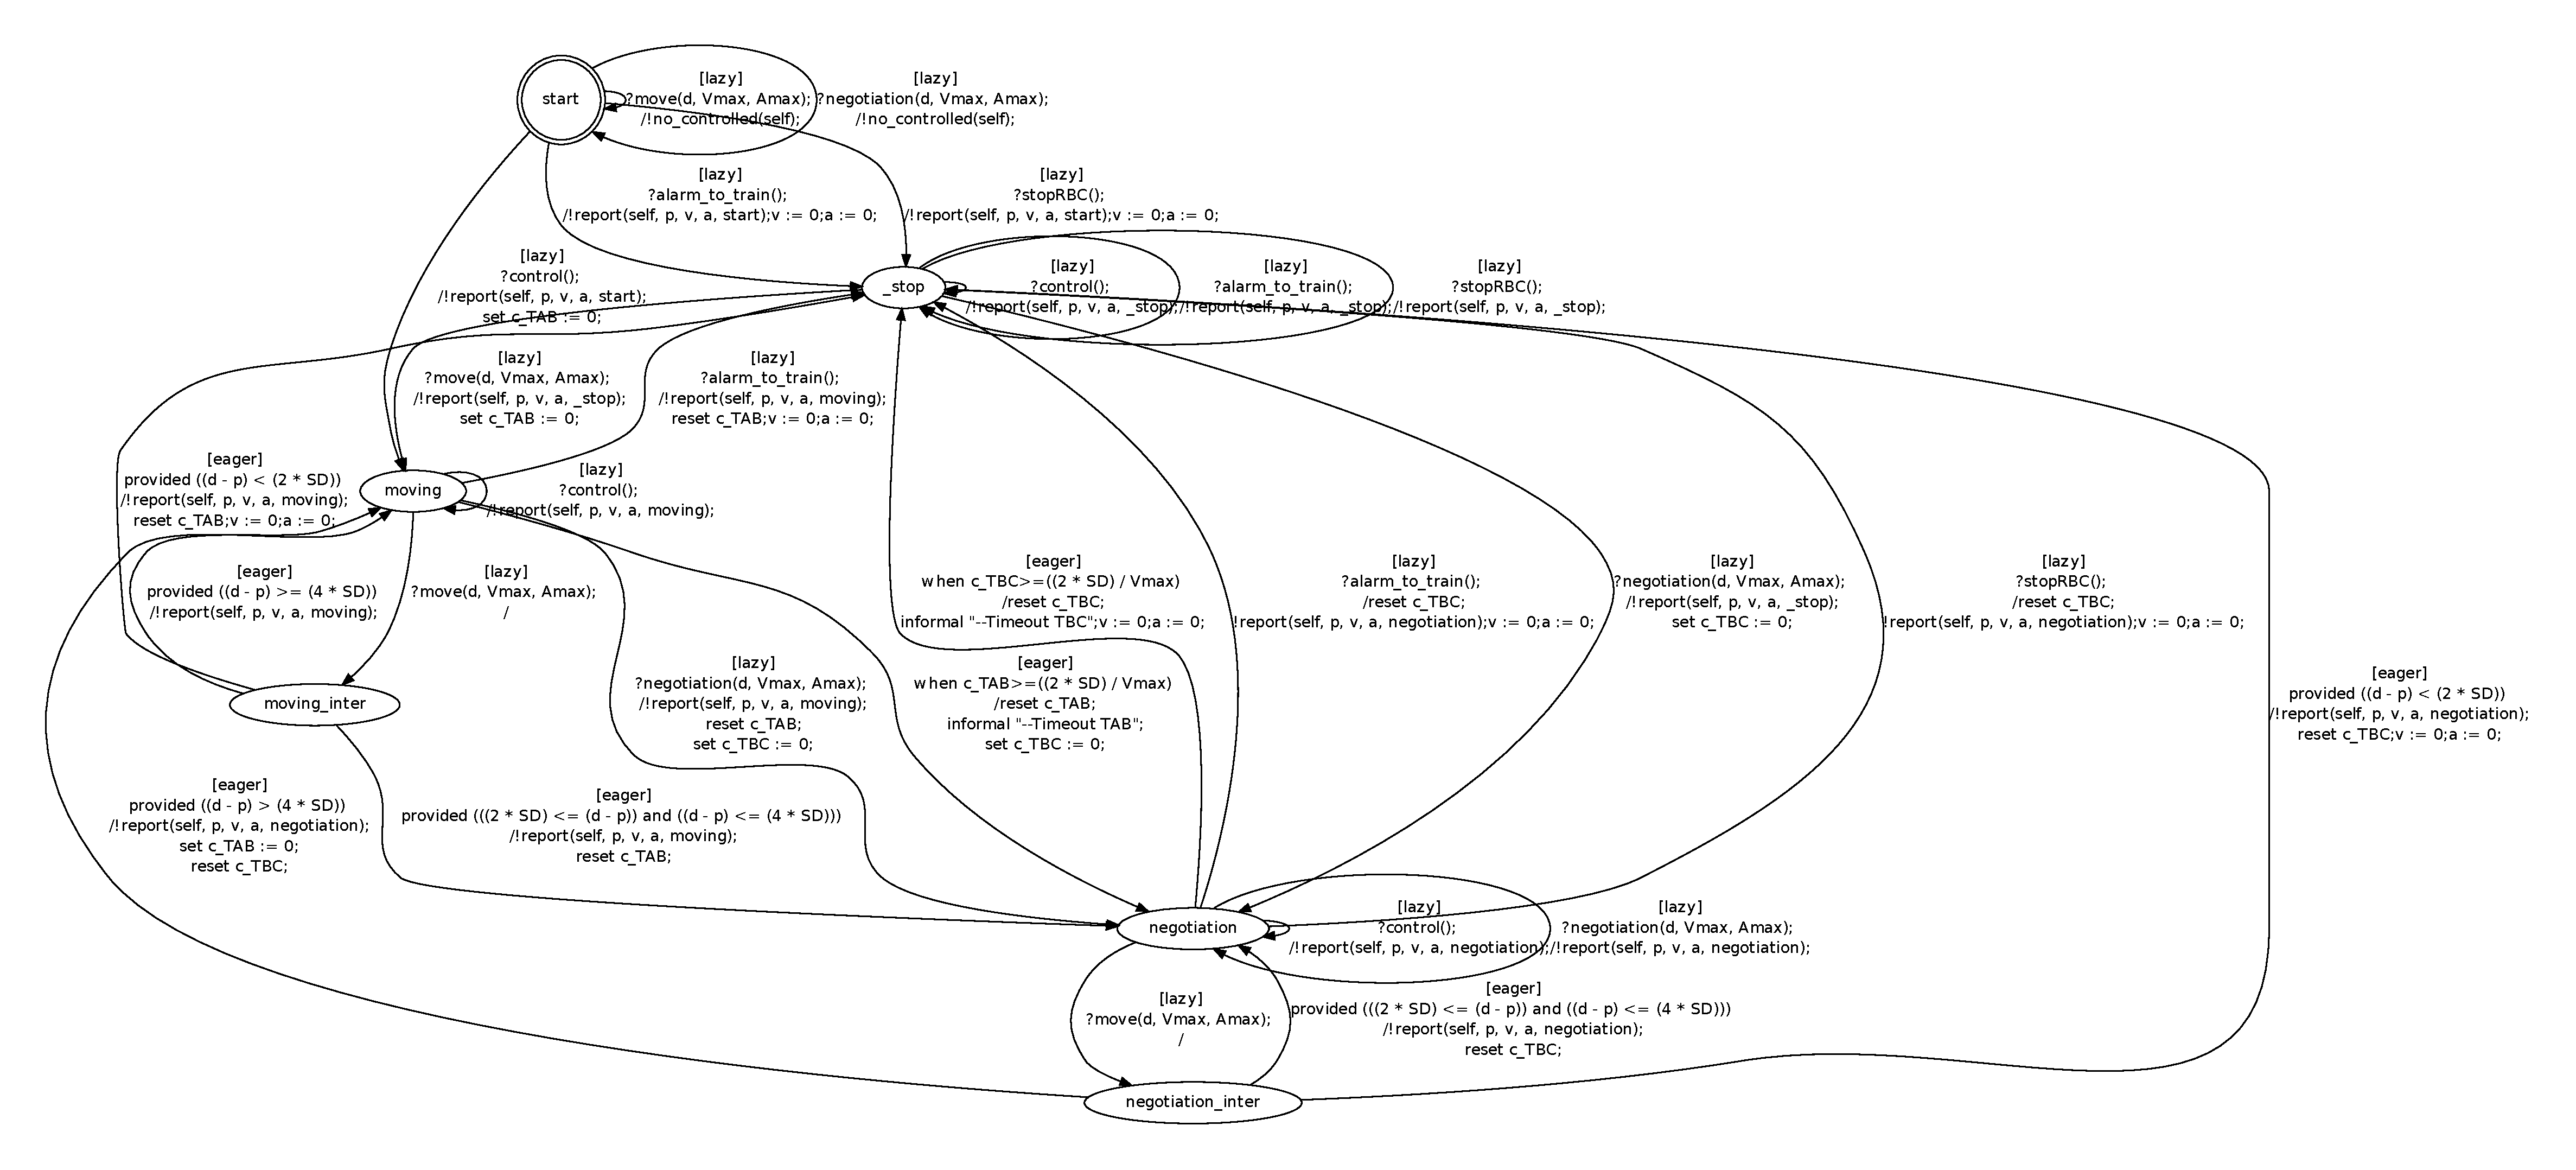
\includegraphics[width=24.5cm, angle=90]{figures/if-model.pdf}
  \caption{Extended Timed Finite State Machine of OBU}
  \label{fig:model}
\end{center}
\end{figure}



The formal model is then represented by IF description% or XML 
in order to be checked by using IF model-checker.
Test cases are generated by using TestGen-IF.

\textbf{Model Checking using IF.}
Model checking is an automatic technique for verifying finite-state reactive
systems. Using such techniques one could automatically check if the model
specifies most of the requirements of the system, such as the important safety
properties described in Task 4.4. Similar to proof techniques, in order to use
model checking to verify if the SFM (Semi-formal model) and FFM (fully formal
model) comply with the safety and function requirements,
the properties to be proven have to be identified and described. To implement
the use model checking, it is mandatory to specify the model using finite-state
reactive systems, and they should also provide an intuitive way to express the
properties to be model checked. The language for describing a formal model for
which corresponding model checkers exist should be selected and the set of
critical requirements to be verified need to be clearly identified. The proposed
model checking techniques should be supported in the selected tool chain. As
mentioned above, we are using IF-based specification to perform
the model checking of train safety properties.


\subsubsection{Results}



\paragraph{Summary}

We have provided a method to formally model the
movement authority requirements of the train using
finite state machines augmented with continuous variables (train position, speed, acceleration) and
time constraints. 

We have modeled OBU on Timed Extended Finite State Machine.
We have then used IF model checker to verify the
proposed formal model. 

During the modeling we discovered 3 inconsistencies, ambiguities and gaps in the specification
which we reported in~\cite{specfindingsTSP}.

\paragraph{Conclusions/Lessons Learned}

Currently, the obtained model can be considered as an abstract representation
of the system specification provided by the standard, i.e., the MOVE
function mode of the OBU can be refined to SHUNTING, TRIP function modes of
OBU in Subset-026.4.4.


\subsubsection{Next Steps}

On the one hand, we refine our formal model to take into account different
function modes of OBU.
In the other hand, we complete the automatic translations from the SysML
specification to the IF specification or to our Java simulator.

%%%%%%%%%%%%%%%%%%%%%%%%%%%%%%%%%%%%%%%%%%%%%%%%%%%%%%%%%%%%%%%%%%%%%%%%%%%%%%%%%
\subsection{Verification on Java simulator}

\subsubsection{Object of Verification}
Model of the Movement Authority converted from IF language to the simulator.

\subsubsection{Available Specification}
Conversion of the IF model described on the previous section.

\subsubsection{Detailed Verification Plan}

\paragraph{Goal} 
We intend firstly to model the Movement Authority of OBU described in
Subset-026-3.8. We then use the model to validate the safety
properties and to generate the test.

\paragraph{Method/Approach}

\paragraph{Means}

\textbf{Test Generation using TestGen-IF.}
When using model checkers the criteria for the model to be safe is that all the
safety properties should be checked. This is impossible, since the number of
safety properties could be infinite and thus, only some of them can be checked
through the above step.
For this reason, as a complementary approach, testing is commonly used. If the
corresponding model respects some requirements, i.e., only expected outputs are
produced to applied input sequences, to some extent, there is a confidence that
the models is safe. In order to derive ‘good’ tests a formal model should be
involved. It is known that only the FSM model where each input is followed by a
corresponding output allows automatic deriving finite tests with the guaranteed
fault coverage where the races between inputs and outputs can be easily avoided.
 Many authors for deriving finite tests with the guaranteed fault coverage turn
their model to some kind of an FSM (see,
e.g.,~\cite{springintveld2001testing,zymc11,Gromov2009}).

We decided to use TestGen-IF to automatically extract a set of test cases from
the formal model described in the IF language. We have identified a set of basic
requirements and we can describe them as IF properties.  Based on these
properties, the TestGen-IF tool automatically generates a set of test cases.
These test cases can be used to test if the model follows the requirements defined for the test generation.

\textbf{Adaptive Testing of Java simulator.}
For simulation, the artifacts should provide means to execute the model.  The
simulator must be automatically generated, so that, when run against test
scenarios (inputs/outputs for the model), we may conclude whether the model
follows the specification or not. In particular, it is important to define test
scenarios for the safety critical properties. The simulation should cover all states,
transitions, data-flow, and paths in the model. It would also be desirable to
include graphical representation of the simulation/model and also provide a
report of the visited components. Being able to trace the
requirements that are met during a simulation is also advisable to allow simple
requirement coverage.

Once we have a test suite generated by TestGen-IF, we execute them using our simulator. The simulator provides a trace of the execution of each test and the expected trace. By comparing both traces it is possible to identify problems with the model.


\subsubsection{Results}

\textbf{Summary}

We have provided a method to formally model the
requirements of the European Train Control System using finite state machines
augmented with continuous variables (train position, speed, acceleration) and
time constraints. 

We have modeled OBU on Timed Extended Finite State Machine.
With TestGen-IF we automatically generated a test suite that was used to verify our simulator.
%

\textbf{Evidence Produced}

By providing TestGen-IF with test objectives, we were able to automatically generate a test suite capable of verifying the properties related to them. Currently we have four different test objectives and with them we generated a suite of 22 tests. By providing more test objectives it is possible to generate more tests.
Each test constitutes a sequence of inputs (or period of time without an input) and expected outputs.

The tests generated were executed by the simulator. When executing a test, the simulator provides a file that compares the expected trace with trace that was simulated. If an inconsistency occurs, the test is considered failed. On our first execution we found some inconsistencies between the IF model and the model used by the simulator. After taking care of these inconsistencies we were able to execute all the tests pass.

\paragraph{Conclusions/Lessons Learned}
It is possible to find inconsistencies in a model using the Java simulator to execute tests. However, further testing is needed to determine the completeness of our test suite.

\subsubsection{Next Steps}
We plan to verify the fault coverage of these tests by executing Java
simulator against corresponding traces and Java Mutants. For this stage we used an older version of the model. A newer version is currently being updated and will be used on future activities.

\newpage


\let\oldparagraph\paragraph
\let\oldsubparagraph\subparagraph

\renewcommand{\paragraph}[1]{\subsection{#1}}
\renewcommand{\subparagraph}[1]{\subsubsection{#1}}

\section{TWT GmbH Science \& Innovation: Verification of Procedures of Subset
026-5}

This sections reports on the modeling of the procedures described in Subset 026, Chapter 5---that is, the behavioral part of the ETCS. The goal of the activity is to validate the specification and to support the modeling using SCADE and the verification of SCADE models on a higher\footnote{in comparison to SCADE models} level of abstraction.

The activity is described in the Verification and Validation Plan (see Sect.~6.1.2.5). In short, we provide feedback regarding ambiguities, inconsistencies and errors in the current ETCS standard based on our formalization of the specification using mathematical modeling languages.

\paragraph{Object of verification}

The object of verification is Subset 026-5 of the specification. We formally model parts of the specification and use the resulting model to validate the specification. This design step has been described in D2.3 (see Sect.~4.4).

\paragraph{Available specification}

The specification is described in Subset 026-5. It describes procedures of ETCS entities (i.e., required reactions on events and received messages), thereby focusing on required change in status and mode of entities considered.


\paragraph{Detailed verification plan}

\subparagraph{Goals} 

The goal is to model the the procedures described in Subset 026-5, thereby focusing on modeling the \textit{system behavior}---that is, the control flow of the on-board unit and the interplay with its environment (e.g., the driver and the RBC). The model is then used to validate the specification.

\subparagraph{Method/Approach}

As a formal model, we use \textit{colored Petri nets} (CPNs)~\cite{CPN-book}, an extension of classical Petri nets~\cite{PNbook} with data, time, and hierarchy. CPNs are well-established and have been proven successful in numerous industrial projects. They have a formal semantics and with CPN Tools~\cite{Westergaard2013apn}, there exists an open source tool for modeling CPNs. Moreover, CPN Tools also comes with a simulation tool and a model checker, thereby enabling formal analysis of CPN models. 

We focus on modeling the \textit{system behavior}---that is, the control flow of the on-board unit and the interplay with its environment (e.g., the driver and the RBC). Figure~\ref{fig:Top} depicts the CPN representing the highest level of abstraction. It shows the decomposition of the overall system into the on-board unit and its environment: the driver, the RBC, the RIU, the STM, and the GSM module. Each component is modeled as a subpage (i.e., a component). Graphically, a subpage is depicted as a rectangle with a double-lined frame. Furthermore, the model shows through which message channels and shared variables the on-board unit is connected to its environment. A channel or shared variable is modeled by a place which is graphically represented as an elipse. As an example, the driver (i.e., subpage \texttt{Driver}) may send a message to the on-board unit (i.e., subpage \texttt{On-board Unit}) via the place \texttt{msg from driver}, and receives messages sent by the on-board unit via the place \texttt{msg to driver}.

\begin{figure}[tb]
	\centering
		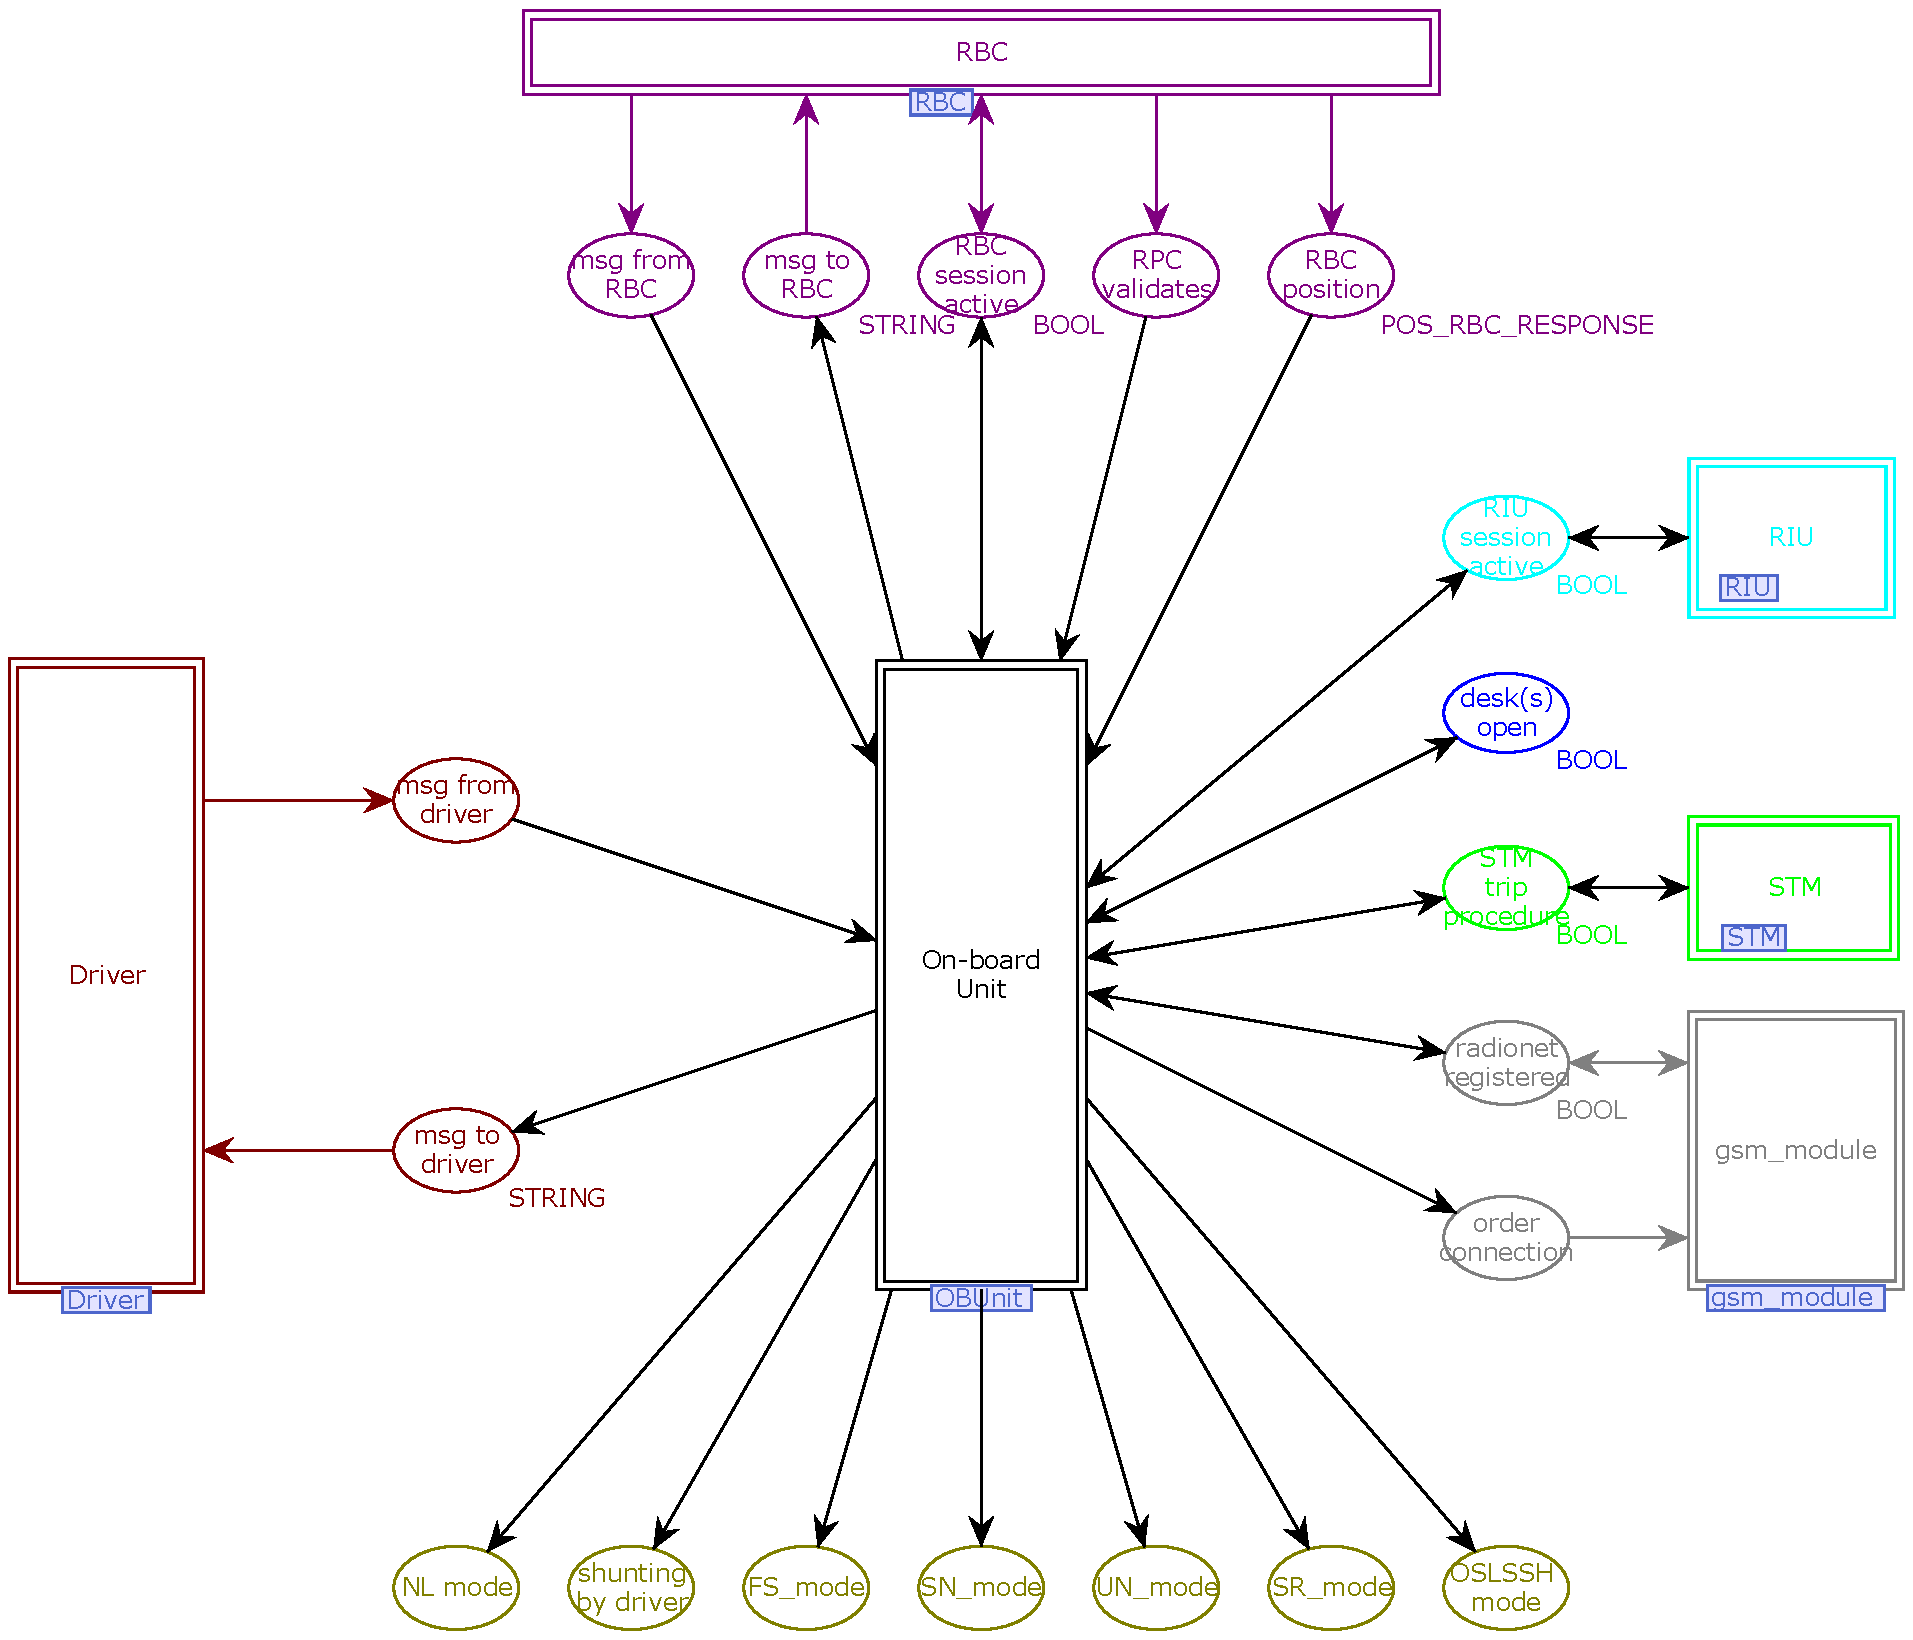
\includegraphics[width=0.9\textwidth]{figures/Top.pdf}
	\caption{Top level model}
	\label{fig:Top}
\end{figure}

Zooming in subpage \texttt{On-board Unit} yields the CPN model in Fig.~\ref{fig:OBUnit}. This CPN model has two subpages: Subpage \texttt{Start} models the states S0 and S1 of the specification (i.e., Subset 026-5.4) and subpage \texttt{Rest} the remaining states. At this level of abstraction, we see on the left hand side seven places (green frame). Each such place models (a part) of the state of the on-board unit, for example, the mode and the train running number. The current model has 689 places, 173 transitions and 1,227 arcs.

\begin{figure}[tb]
	\centering
		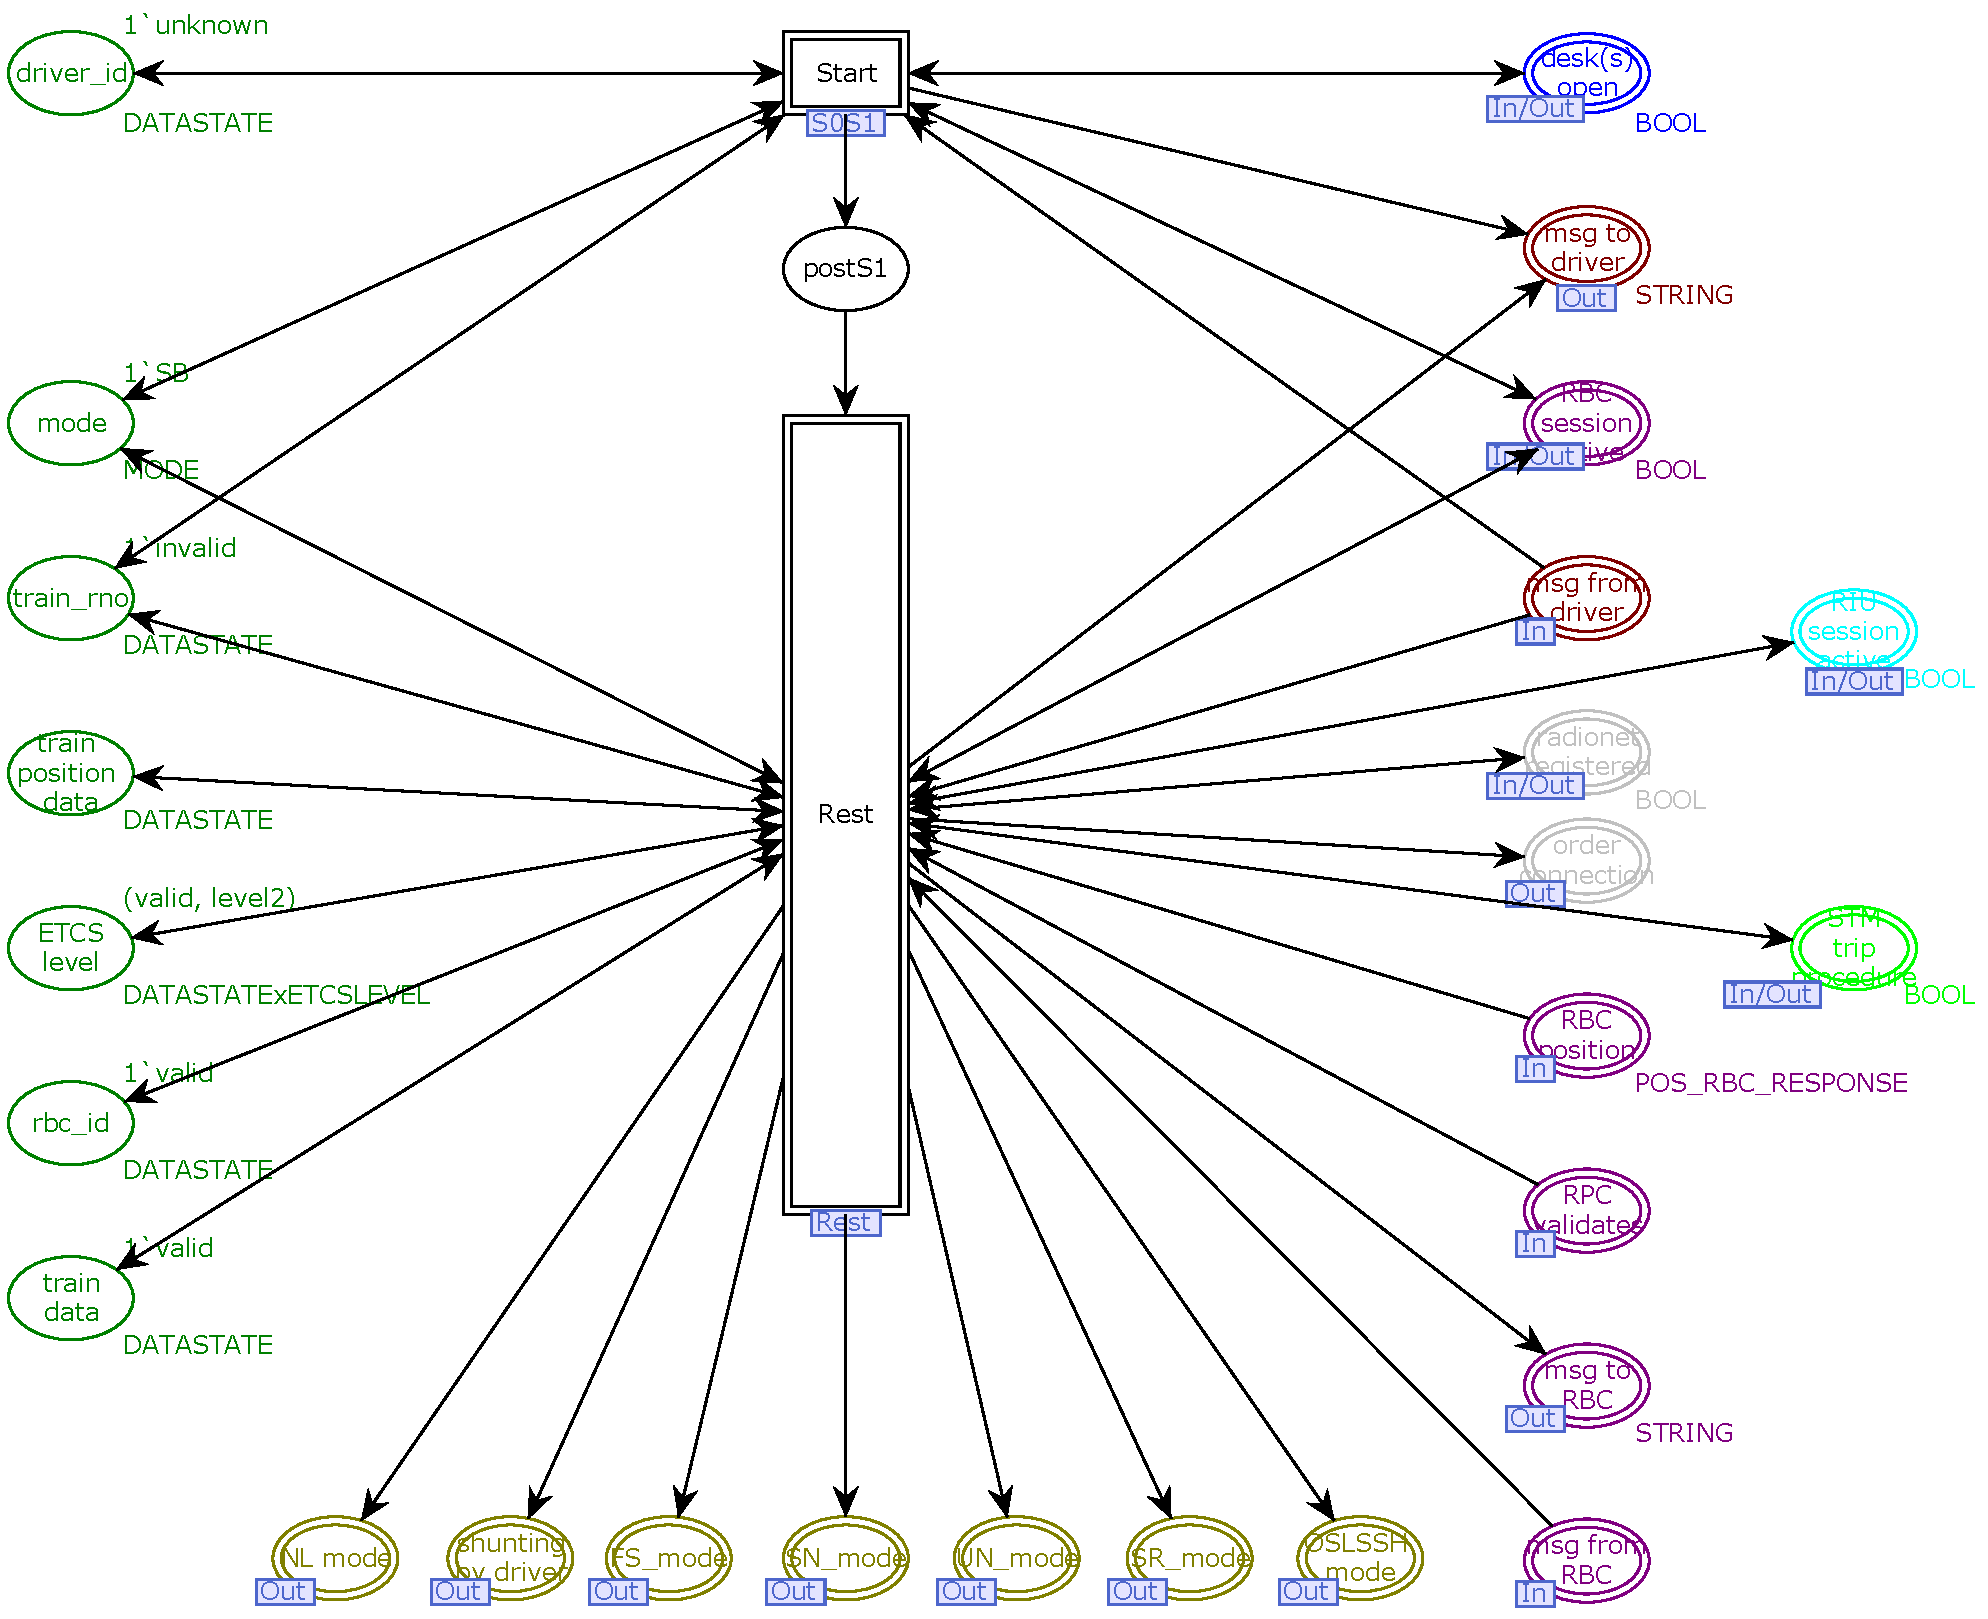
\includegraphics[width=0.9\textwidth]{figures/OBUnit.pdf}
	\caption{CPN model of the on-board unit}
	\label{fig:OBUnit}
\end{figure}

Having a more detailed look at Fig.~\ref{fig:OBUnit}, we observe that our model does not represent all variables of the on-board unit as given in the specification and also partially abstracts from data. We abstract from those details, because the model is tailored to formalize the \textit{control flow} of the on-board unit and, in particular, the \textit{communication behavior} with its environment. As a benefit, this abstraction reduces the complexity of the model and improves its understandability. Additional details, such as data and precise message values, can be added in a refinement step.

The modeled procedures have been manually modeled using CPN Tools. Thereby, each element in the model has been reviewed against the respective requirement, as given in the specification. To improve the confidence in the model, in a second step, a person other than the modeler checked the model against the specification. In addition, we used the simulator to check whether the modeled behavior of the CPN matched the intended behavior.

So far, the primary goal of modeling has been to validate the specification. During the modeling we discovered 36 inconsistencies, ambiguities and gaps in the specification which we reported in~\cite{specfindings}. 


\subparagraph{Means}

The input for our approach is the specification described in Subset 026-5. Our output is a CPN model and a report describing inconsistencies, ambiguities and gaps in the Subset 026-5.


\paragraph{Results}

\subparagraph{Summary}

We have modeled the following five procedures of Subset 026-5 as CPN:
\begin{itemize}
	\item Start of Mission (Subset 026-5.4)
	\item End of Mission (Subset 026-5.5)
	\item Shunting Initiated by Driver (Subset 026-5.6)
	\item Override (Subset 026-5.8)
	\item Train Trip (Subset 026-5.11)
\end{itemize}
During the modeling we discovered 36 inconsistencies, ambiguities and gaps in the specification which we reported in~\cite{specfindings}. Our CPN models the system behavior---that is, the interplay between the different entities of the ETCS---and partially abstract from data. Therefore, we complement the work on SysML modeling, where the focus is on the connectivity of components and the data types.
 
\subparagraph{Conclusions/Lessons learned}
 
The numerous specification findings illustrate the need for validating the specification. CPNs are well-suited to model the behavioral aspects described in Subset 026-5. The size of the model clearly indicates the complexity of the procedures, even at the current level of abstraction. Therefore, we expect that applying formal verification on the resulting CPNs will not be feasible due to state-space explosion.

\paragraph{Future Activities}


We shall continue our work by completing the model, contributing to the modeling of (parts of) Subset 026-5 using SCADE, and verifying the SCADE model. In addition, we are planning to exploit synergies by collaborating with the project partner LAAS who advocate the Petri net model checker TINA~\cite{BerthomieuV2006}. In addition, we are working with the project partners from Braunschweig University of Technology on generating test cases from the CPN model.


\paragraph{Modeling the Subset 026-5}

We plan to model the remaining parts of Subset 026-5, thereby reporting possible additional findings in the specification. The goal is to have a CPN modeling all procedures that are described in Subset 026-5. We also want to compare our model with the (corresponding part of the) ERTMSFormalSpec model~\cite{ertms}.


\paragraph{SCADE Modeling}

As the ETCS will be modeled using SCADE, we shall contribute to this modeling process. To use the experience that we gained from modeling Subset 026-05 with CPN Tools, we want to contribute to the SCADE modeling of (parts of) the Subset 026-5. The SCADE design flow starts with modeling all components and their interplay using SysML block diagrams (with the tool SCADE Designer). The resulting SysML diagrams provide a functional and an architectural view. They are similar to the CPN model in Fig.~\ref{fig:Top}. In a second step, the behavior of each block has to be fully modeled on the system level using SCADE Suite. Currently, SCADE does not support state machine models on the level of SysML. Our CPN model provides this level of abstraction and will, therefore, be useful for the SCADE modeling.


\subparagraph{Verification of the SCADE Model}

Another task concerns the verification of the resulting SCADE model. Recently, researchers reported on complexity problems already for medium-sized SCADE models that restrict the verification using the SCADE prover~\cite{HuhnM2014scp,DaskayaHM2011fmics}. Given the complexity of the ETCS, we assume that we will face similar challenges. To alleviate those complexity problems, we aim to apply the following three techniques:

\begin{description}
	\item[Abstraction:] We will apply abstraction techniques on the SCADE model to prove safety properties on a higher level of abstraction whenever possible. On the one hand, we can apply SCADE contracts to restrict the domain of the input values. This technique is known as environment abstraction. On the other hand, we can transform the SCADE model into a model of higher abstraction, thereby using different formalisms such as timed automata, transition systems and Petri nets. (As SCADE has a formal semantics such transformations are possible, but may take considerable effort.) We can then use verification tools that are dedicated to the properties of interest and the chosen formalism. We see the chance that our CPN model can be used for this task, too. For example, Uppaal~\cite{BehrmannDLHPYH2006} can analyze timed automata, the Spin model checker~\cite{Holzmann97} and NuSMV~\cite{CimattiCGGPRST2002} can analyze transition systems, and TINA~\cite{BerthomieuV2006}, LoLA~\cite{Wolf2007}, and CPN Tools~\cite{Westergaard2013apn} are tools for analyzing (different variants of) Petri nets.
	%
	\item[Compositional Reasoning:] Another approach is to prove properties for individual components and deduce from it the correctness of a property concerning the entire ETCS. Here we think that we can, in particular, combine our model with the MoRC model~\cite{braunstein_MorC_2013} and apply compositional reasoning.
	%
	\item[Correctness by Design:] The two previous approaches support \textit{correctness by verification}; that is, first the model is designed and in the next step it is verified. A different methodology is \textit{correctness by design}. The idea is to model on a higher level of abstraction and to prove that certain safety properties hold. Then the model is iteratively refined. Each refinement step has to guarantee that all properties that hold for the more abstract level also hold in the refined model. The challenge is to find property-preserving refinement rules or a refinement relation between an abstract model and a refined model that preserves the desired properties and to verify that this relation holds. The results can be applied to validate the SCADE model and the specification.
\end{description}





\newpage


\newcommand{\tbi}[1]{$<$\textit{#1}$>$}

% Starts a new line nearly everywhere
\newcommand{\nl}{\mbox{}\\}
\newcommand{\nlskip}[1]{\mbox{}\\[#1]}

%
%Comments
\newcommand{\cmmnt}[1]{\framebox{#1}}
\newcommand{\bgcmmnt}[1]{\nl\framebox{\parbox{.95\textwidth}{#1}}\nl[2mm]}
%\renewcommand{\bgcmmnt}[1]{}
%

\newcommand{\eod}{\nl\rule{.95\textwidth}{1pt}\nl\textit{End of Document}}


\section{University of Bremen: Verification of the  Management of the Radio
Communication}
\label{sec:ubremen}
This section reports the verification activity of SCADE-MoRC. The goal
of this activity is, first, to establish the compliance of the SCADE
model to the SRS description via testing. Secondly, we want to track
the ambiguities within the specification. Finally we want to
demonstrate the efficiency of model based testing using the RT-tester
tool for system integration testing.

The activity is described in the Verification and Validation Plan
section {\em 6.1.2.7 System Integration Testing (Uni Bremen/DLR)} \cite{D4.1_2013}.
In short, we develop a test model from the specification, generate tests and use
the code generated from SCADE to perform software-in-loop testing.
The test model and the SCADE model used to generate code have been
done independently to each other. 

\paragraph{Object of verification}
 Management of radio communication (MoRC) ERTMS function baseline 3.


The system under test (e.g. the verification object) is the C code
generated from a SCADE model and described here
\url{https://github.com/openETCS/model-evaluation/tree/master/model/SCADE_Siemens/Subset_026_Chapt_3.5_ManagementOfRadioCommunication/Generated_C_Code}.
It describes the Management of the radio communication at the software
phase.




\paragraph{Available specification}

The specification is described in the
Subset-026 chapter 3.5. It
describes the communication protocol between the EVC and the RBC or
balises. In particular, how the EVC initiates and terminates a
communication.



\paragraph{Detailed verification plan}

\subparagraph{Goals}

To achieve what has been defined previously a test model in SysML has
been developed. The description of this verification artifact may be
found here \url{https://github.com/openETCS/model-evaluation/blob/master/model/EA-SysML/new_version/doc/ea_sysml_report.pdf}

Our main goal is to verify the SCADE model by test simulation. The
tests are produced by a model of the Subset-026 chapter 3.5 described as a
state machine.

\subparagraph{Method/Approach}

\begin{figure}
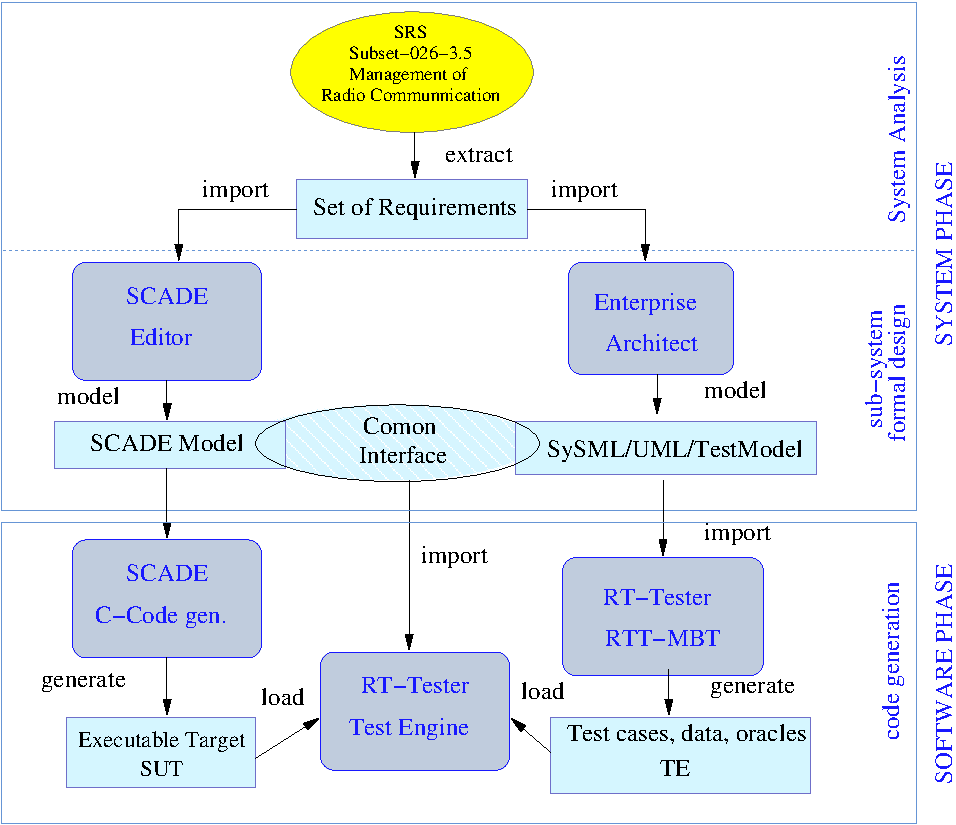
\includegraphics[width=\textwidth]{schema/framework}
\caption{\label{fig:method}SCADE/RT-Tester methodology}
\end{figure}

Figure \ref{fig:method} depicts our methodology. From the SRS
specification, two models are designed: one SCADE model that will
be then  used to produce C code and one SysML model for generating
tests.

Our test model contains the behavioral representation of the MoRC, the
set of requirements of the chapter 3.5, and the link between the behavior
and the requirement.  Most of the requirements may be represented as
single transition or state in the test model state
machine. Nevertheless, some of the requirements may be only modeled as
a path of the state machine, we choose to represent those as LTL
formula, added as constraints of the test model. For example the
\verb+REQ-3.5.3.10+ describes the steps needed for the establishment of
the radio communication order by the RBC. This requirement explicits a
particular path of the test model, thus this path should exists in our
test model. To ensure that this particular test will be generated a LTL
formula has been added (See \cite{braunstein_MorC_2013} for more
details).

\begin{description}
\item[REQ-3.5.3.10] "If the establishment of a communication session is
initiated by the RBC, it shall be performed according to the following steps
..."
\vspace{-1em}
\begin{verbatim}
Finally (MessageIn == INIT_SESSION_TRACK && setUp == 1 -> 
Next (MessageOut == SESSION_ESTABLISHED && radioComSession == ESTABLISHED)
\end{verbatim}
\end{description}

We need then to link the system under test and the test model. Since
the two models are elaborated independently, we need to ensure that
the tests generated may be handled by the code generated by SCADE and
conversely we need to read the output of the C code back to the test
generator to compare the values with our oracles. This is achieve by
defining a common interface that the two models should respect. The
inputs drive the tests and the outputs are the observational points to
state if a test pass or fail. Hence, the two models should respect the
same interface.

After the modeling phase, starts the test generation phase.
Two strategies have been used for the tests generation. First, we
generate a set of test following the common behavioral coverage
strategies ensuring the following coverage :
\begin{itemize}
\item  Basic control state coverage (BCS): All state locations are covered.
\item  Transition coverage (TC): All transition of the statecharts are covered.
\item  Modified condition/decision coverage (MC/DC): Modified condition/decision coverage.
\item  Hierarchic transition coverage (HITR): High-level transition of
  nested statecharts are covered.
\item  Basic Control states Pair coverage(BCPAIRS): For concurrent state
  machines pair states of two different state machines. 
\end{itemize}

More detailled explaination on the coverage may be found here \cite{huang_test_2013}.

We then apply a requirement coverage strategy to
generate tests that covers all the requirements. 
As each requirement
is linked to an artifact of the test model, part of the test cases
are generated as subset of the coverage mention above. In addition,
test cases from the LTL are also provided.


Finally the test engines run the SUT with the stimuli from the test
model. In parallel, it runs the test oracles that states if the test
pass or fail.

\subparagraph{Means}

The Artifacts are produced as follow:
\begin{itemize}
\item C code comes from SCADE model.
\item Test model is a SysML model designed with Enterprise Architect.
\item Test cases, tests data and test oracles are generated with RT-tester.
\item Executable code compile with gcc.
\item Code run within the RT-Tester engine.
\end{itemize}

SCADE is EN 50128 qualified at SIL 3/4, RT-tester is also certifiable
T3 as shown in \cite{peleska_efficient_2012}.

\subsection{Results}

\begin{table}[htbp]
\centering
\begin{tabular}{lr}\toprule
  Coverage strategies & \# tests generated  \\\midrule
  BCS & 14 \\
  TC & 40 \\
  MC/DC & 79 \\
  BCPAIRS & 33\\
  HITR & 12 \\
  LTL & 2 \\ \midrule
  Total Tests& 180\\\bottomrule
\end{tabular}

\vspace{1em}
%\raggedleft Total Requirements cover 40
\caption{\label{tbl:test_summary} Test cases generation summary}
\end{table}

Table \ref{tbl:test_summary} resumes the set of automatically
generated tests.
The set of tests cover 40 of the requirements from the chapter 3.5.


The simulation result of the C code is not yet finished and for the
moment, all test failed. The main reason was that the two
models did not share the same starting condition.
Hence, we  need to refined our test model to be able to handle SCADE
modeling style correctly and be able to have interesting result.



\paragraph{Summary}

What we have done:
\begin{enumerate}
\item Created a test model in SysML.
\item Generated test cases.
\item Ran SCADE model against test procedure produces by RT-tester.
\end{enumerate}
 
 The next step:
 \begin{enumerate}
 \item Refined test model
 \item Analyze the result of the test procedure.
 \item Coordinate DLR/SIEMENS/Uni Bremen interfaces.
 \item Run the test on the DLR lab.
 \end{enumerate}

\paragraph{Conclusions/Lessons learned}

Our first attempt to simulate the tests was not a success. All tests
except the one covering the initial states failed. Our two models
have, at least, the same initial state.
From  our first investigation, we could see that one chapter of
the specification is not self-contained. This leads to different
interpretation in the modeling and thus some non equivalent behaviors.

Moreover some missing information in the specification leads to 
 constraints in test model. It affects the test generation by
providing some non realistic test cases. Some variable behavior that
were not mentioned in the specification are considered as free and may have any
possible value in their definition range. This can be solved by adding
information into the test model. 

More precisely, the test model is composed with a system under test
and a test environment. In our first model the test environment is
empty, meaning that all inputs of the SUT are free. The test
enviroment may be described (and constrainted) by statecharts or
LTL formula that restricts the behaviors of the inputs. The test
generator should then find  test suites that realize the given
coverage and that respect the constraints given in the test environment.



\paragraph{Future Activities}
\subparagraph{Refine the test model}
\begin{enumerate}
\item Analyze the test results of the SCADE C code
\item Enumerates specification ambiguitites: where the two parties did
  not undestand the specification in the same way.
\item Refine the test model by adding a better test environment with
  the help of domain experts
\end{enumerate}
\subparagraph{New activities}
We will also provide the ceiling speed monitoring function to enrich
the test model and apply new model based testing approach.

%\bibliographystyle{plain}
%\bibliography{biblio}



\newpage

%\documentclass{article}
%\usepackage{hyperref}
%\usepackage[utf8]{inputenc}
%\usepackage{graphicx}
%\usepackage{booktabs}
%\graphicspath{{schema/}}
%\title{Performance Estimation of the Speed and Distance Monitoring}
%
%\author{Alexander Nitsch \and Benjamin Beichler}
%\date{\today}
%
%\newcommand{\tbi}[1]{$<$\textit{#1}$>$}
%
%% Starts a new line nearly everywhere
%\newcommand{\nl}{\mbox{}\\}
%\newcommand{\nlskip}[1]{\mbox{}\\[#1]}
%
%%
%%Comments
%\newcommand{\cmmnt}[1]{\framebox{#1}}
%\newcommand{\bgcmmnt}[1]{\nl\framebox{\parbox{.95\textwidth}{#1}}\nl[2mm]}
%%\renewcommand{\bgcmmnt}[1]{}
%%
%
%\newcommand{\eod}{\nl\rule{.95\textwidth}{1pt}\nl\textit{End of Document}}
%
%\begin{document}
%\maketitle
%\begin{abstract}
%  This document reports the verification activities of the University of Rostock. SystemC (performance analysis), executable models: SysML modelling and code generation, Scade modeling and code generation.
%\end{abstract}


\subsection{Verification of the Speed and Distance Monitoring}

This section reports the verification activities of the \emph{Speed and Distance Monitoring} with model based simulation and virtual prototyping. The first activity pursues the goal of formalizing the specification in the form of an executable model. This model provides a performance estimation at an early stage of system level design and adduces evidence what hardware resources will be needed for the future OBU. Secondly, finding and reporting of unclarities, inconsistencies, incompleteness and errors while implementing the specification by using tools of the openETCS toolchain (Papyrus/SysML, SCADE). Furthermore, we are developing a method of SystemC code generation from abstract and domain specific SysML models. Finally we want to demonstrate the efficiency of model based simulation after transformation from SysML to SystemC models.

The activity is described in the Verification and Validation Plan
section {\em 5.3.10 Verification with Model-Based Simulation} \cite{D4.1_2013}
To sum up, we develop application models from the specification of the \emph{Speed and Distance Monitoring}, generate test scenarios and use the inherent simulation environment of SystemC to do performance and scheduling analysis.

\paragraph{Object of verification}  Speed and Distance Monitoring ERTMS function baseline 3.
The system under test is the implemented SystemC code which is described here: \url{https://github.com/openETCS/model-evaluation/tree/master/model/SystemC_TWT_URO/3.13_Speed_and_distance_monitoring}. It describes the Speed and Distance Monitoring at the Software phase.
\nl

\begin{figure}[h]
\centering
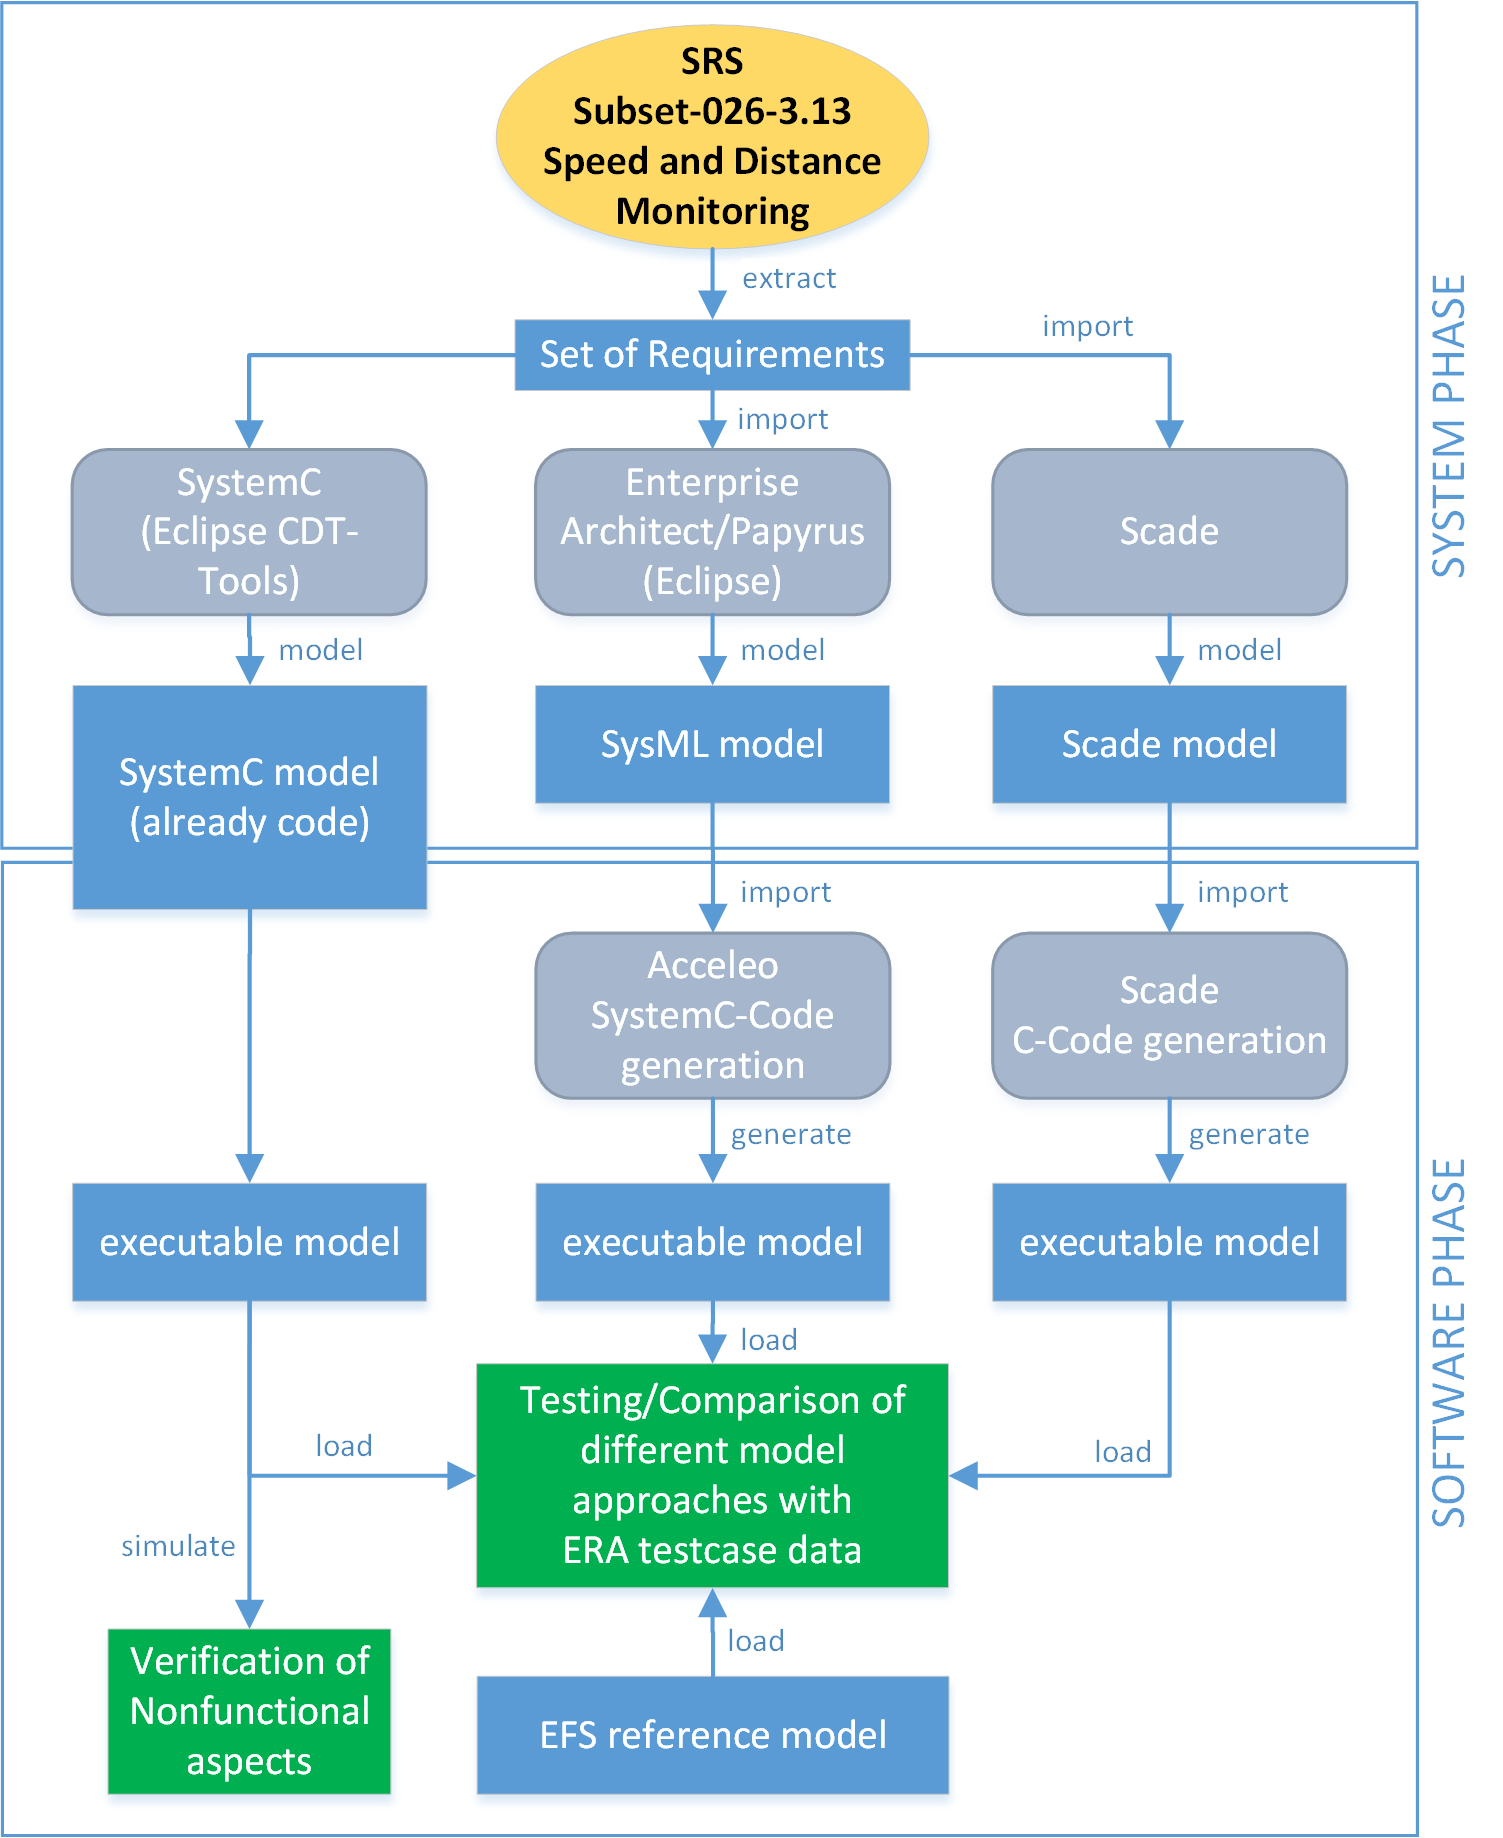
\includegraphics[width=.80\textwidth]{schema/UniRostockApproach.png}
\vspace{4mm}
\caption{University of Rostock VnV Approach}
\label{fig:University of Rostock VnV Approach} 
\end{figure}

\paragraph{Available specification}

The specification is described in the
SUBSET-026 Chapter 3.13 \cite{unisig_subset-026_2012}. It describes the realization of both TI and DMI commands by calculating several modules with inputs form train side, track side an odometry. The University of Rostock focuses on the calculation of parts, which are used for safety critical cases using emergency brakes. This especially includes the EBD (emergency brake deceleration) curves.

\paragraph{Detailed verification plan}

\subparagraph{Goals}

On the one hand we are testing extra-functional aspects such as performance and scheduling analyses to give evidence which hardware system is sufficient to meet the system requirements. We want to discover which hardware resources (e.g. number of processors) will be needed for the OBU. This is important to avoid excessive delays to ensure adequate response times in critical situations. Therefore the University of Rostock will do model based simulation using the inherent simulation environment of SystemC.

On the other hand we use the existing SystemC model to check against a reference model, such as EFS braking curve model. Furthermore we use different tools and means to build additional system models for comparison and verifying behavior.

\subparagraph{Method/Approach}

Figure \ref{fig:University of Rostock VnV Approach} depicts our methodology. Three models will be created from the SRS
specification: one SystemC model that is directly implemented into executable code (finished), one SysML model that will be used to produce SystemC code to be executable (not finished) and one SCADE model that will be used to produce C code (not finished). For model verification we use test cases and data provided by WP4 and use the ERA excel datasheet as reference implementation. The created test models will contain behavioral representation of the \emph{Speed and Distance Monitoring} such as state machines, activity diagrams and sequence diagrams. There will be a link to the specification requirements to meet the needs of traceability in terms of verification activities.


\subparagraph{Means}

The Artifacts are produced as follow:
\begin{itemize}
\item SystemC code which is directly implemented.
\item One Test model is the SystemC model. It's code will be generated/transformed by Acceleo from abstract SysML models designed with Enterprise Architect and/or Papyrus.
\item C code is produced by Scade using Scade System.
\item Executable code is compiled with GNU-C-Compiler \texttt{gcc}.
\item Reference model delivered by ERTMS Formal Specs.
\item Testdata and testcases are provided by ERTMS Formal Specs using the ERA excel data sheet.
\end{itemize}

\subsection{Results}

Verification of extra-functional aspects is successfully done for the first iteration of application models. The provided results consist of recommendations on how hardware resources shall be allocated to the future OBU. The modeling activities are still in progress.

\subparagraph{Summary}

What we have done:
\begin{enumerate}
\item Created an executable model in SystemC.
\item Ran simulations on single, dual and multi core virtual prototypes.
\item Architecture SysML model of the \emph{Speed and Distance Monitoring}.
\item Architecture Scade model of the \emph{Speed and Distance Monitoring}.
\item Defined a reduced set of parameters for calculating braking Curves especially EBD curves.
\end{enumerate}
 
 The next step:
 \begin{enumerate}
 \item Finishing model activities on SysML and Scade.
 \item Developing a model transformation/code generation from SysML models.
 \item Defining an exchanges interfaces between different model approaches.
 \item Run the tests.
 \end{enumerate}
\subparagraph{Conclusions/Lessons learned}
From the first results, we see that SysML is a very powerful graphical modeling language but to perform code generation it is necessary to have restrictions to it. We will have a domain specific SysML profile to get reliable results from code generation.  


\paragraph{Future Activities}
Simulink as a modeling tool is in our interest because there is a bridge to Scade. Simulink provides code generation for hardware description languages such as VHDL. That enables new hardware test scenarios.

\newpage


\let\paragraph\oldparagraph
\let\paragraph\oldsubparagraph


\section{Systerel}

Three approaches of VnV  on formal models have been experimented and are
presented in this section:

\begin{enumerate}
\item VnV on classical B  model that cover software design level, in the objective to provide an open-source approach;
\item VnV on Event-B model that cover system level and support safety analysis;
\item VnV on Scade model that cover software design level.
\end{enumerate}

Classical B and Scade model specify the same example of Subset 026 "§5.9
Procedure on-Sight", Event-B model specifies the "Mangement of Radio
communication" function.

\documentclass{article}
\usepackage[utf8]{inputenc}
\usepackage{amsmath}
\usepackage{url}
\usepackage{amsfonts}
\usepackage{graphicx}

\title{Verification and validation of B~models}
\author{Benoît~Lucet\\Systerel}
\date{\today}

\begin{document}

\maketitle

\begin{abstract}
This document describes the verification and validation processes applicable to B~models. It supports B as a promising method in the context of openETCS, given the maturity and level of rigor associated with it.\\
After an introductory section where we discuss the subject of validation, section \ref{sec:processes} presents the different verification processes and discusses their advantages and drawbacks, while section \ref{sec:tools} presents the tools available to perform such verification. Finally, appendix \ref{app:osproc} presents the application of the verification process to an existing B example: the procedure on-sight.
\end{abstract}

\newpage

\tableofcontents

\newpage

\section{Introduction}
\label{sec:intro}
A B~model is a textual and formal specification covering the functional behaviour of a safety critical software. It is usually written based on a high-level specification (informal or formal specification, for example SysML or a natural language). It is gradually refined, starting at the top with an abstract notation and ending at the bottom with sequential instructions --- which are then auomatically translated in a target language such as C or Ada.\\
Thus, we define three objects of verification and validation: the specification, the B~model and the generated source code.\\

Validation consists of:
\begin{itemize}
\item guaranteeing the functional adequacy between the specification and the model (this can be achieved, for example, through review and proofreading),
\item building a test environment around the generated source code and test it.
\end{itemize}
Hence, this document will mainly focus on verification, i.e.\ the methods and tools required to assure that B~method is a consistent way of producing critical software.

\section{Verification processes applicable to a B~model}
\label{sec:processes}
In this section, we demonstrate the suitability of the B~method towards the problematics encountered in the openETCS project by introducing the different verification processes applicable to a B~model.\\
Each of the verification process is presented and its contributions to the system security and consistency are discussed.

\subsection{Type checking}
Static type checking (TC) is a basic form of program verification that ensures type safety of the model. It is the first verification --- after lexical and syntactic analysis --- to be performed on a B~model, thus allowing an early detection of problems. It is also a pre-requisite for the higher-level verifications. \\
Strong typing ensures a consistent use of data and is essential to writing correct formulae (predicates or expressions).\\

The type checking process consists of two main activities: data typing and type verification.\\
{\itshape Data typing} is the activity of assigning a type to newly-encountered data in a predicate or a substitution\footnote{In B, a substitution is comparable to a set of instructions that modify variables. For more information, see \cite{bbook}.}. It is based on an inference mechanism, which is able to deduce the type of a newly-encountered variable from the type of the other variables intervening in the predicate or the substitution, and specific inference rules.\\
On the other hand, {\itshape type verification} is the activity of verifying typing rules between already-typed variables. These rules are specific to their applying predicates, expressions or substitutions.
% In B, the base types consist of integers, booleans, strings, abstract sets and enumerated sets.\\
% The construction of more complex types is achieved through the powerset operator $\mathbb{P}$ and the cartesian product $\times$.

\subsection{B0-check}
The B0 verification has the specific purpose of checking the respect of the rules that the B~model has to conform to in order to generate the translation to C or ADA. These rules are called implementability rules and must be respected in order for the translation to process properly. They also ensure that the resulting code is executable and respects a set of properties.

\subsection{Well-definedness}
An expression is well-defined (WD) if its associated value or interpretation exists and is unique, thus avoiding ambiguity.\\
Examples of ill-defined formulae include division by zero, function application to an argument out of the domain, function application of a relation etc.\\

Well-definedness checking is thus an extra verification that helps strenghten the model.

\subsection{Model checking}
Model checking is a static semantic check that searches for invariant or assertion violations and deadlock states.\\
This type of verification animates the model, modifying the current state of the machine, starting from the initialization. Operation calls are simulated and modify the internal state which is then checked for various properties. Most of the time, an invariant or assertion violation is looked for.\\

This verification process, as opposed to the ones previously introduced, considers the semantics of the model and aims at verifying properties dynamically. However, it has its limitations:
\begin{itemize}
\item unability to run through all of the states and transitions,
\item difficulty to deal with infinite sets.
\end{itemize}
This means that potential erroneous states can be missed, and that this verification process is not sufficient to ensure {\itshape correctness}, though satisfying as an additional verification tool.

\subsection{Constraint-based checking}

Constraint-based checking (CBC) is the process of finding a given valid state, for which an operation call leads to an erroneous state. This is done by constraint solving instead of --- as seen for model checking --- running through states from the initialization.\\
This technique will usually provide more counter-examples than model-checking, because it ignores the initialization constraints and can thus reach a wider range of states.

\subsection{Formal proof}
A proof obligation is a mathematical lemma generated by the proof obligation generator (POG). It corresponds to a consistency property of the model, that has to be demonstrated.
A fully-proved model is said to be {\itshape correct}, in the sense that every property (invariant, assertion) expressed is proved to hold for every state of the program. If a proof obligation is not provable, it means that the B~model is inconsistent and must be corrected. In fact, the goal of any B development is to obtain a proved model.\\
In contrast to model-checking, formal proof does not require to make assumptions about the size of the system (number of transitions). It is reliable and powerful, but it needs to be taken into account that:
\begin{itemize}
\item some proofs can be very difficult to solve,
\item the model needs to be written as to make it the simplest to prove, which demands experience and skill.
\end{itemize}
A proved model will always meet the safety and security qualifications~; however that doesn't mean it will behave in regards to the specification! This is the domain of validation, as discussed in the introduction.

\section{Tools for verification}
\label{sec:tools}

\subsection{Existing tools}
In this section, we present the existing tools suitable for the verification processes defined in section \ref{sec:processes}.

\subsubsection{Atelier~B}
\label{subsec:atelierb}
Atelier B\footnote{See \url{http://www.atelierb.eu/en}} is the main development tool associated with the B~method and is produced and distributed by ClearSy. It provides most of the needed tools.

\paragraph{B~compiler}~\\
The B~compiler performs syntax analysis, type checking, identifier scope resolution and B0-checking. It is part of Atelier~B as an open source tool.

\paragraph{Proof obligation generator}~\\
Atelier~B's POG is currently the only known fully operational POG for B, and is free of charge --- although proprietary software, which means closed-source. ClearSy is currently working on a new proof obligation generator~; whether it will be open source or not is to be determined.

\paragraph{Prover, proof assistant, user-defined rules}~\\
Atelier~B provides a free of charge --- although not open source --- prover which discharges proof obligations. Depending on the complexity of the model, a varying proportion of the proof obligations is discharged automatically.\\
For the remaining proof obligations, Atelier~B provides an interactive proof assistant allowing the user to guide the prover in discharging the PO. The user may define theories (or rules) which have in turn to be proved. The user-defined rules are organized in a database. 

\paragraph{Atelier~B translators}~\\
Translators are an essential component of the industrial success of B. The translators take the B0 implementations as input and produce a target source code, typically Ada or C/C++, ready to be compiled or integrated in an environment.\\
ClearSy provides an open source translator, but it does not reach the T3 level of qualification\footnote{For additional information on qualification, see subsection \ref{subsec:qualif} or the CENELEC norm.}.

\subsubsection{ProB}
\label{subsec:prob}
ProB is an animator and model checker for B~models distributed under the EPL license (open source) and mainly developed by Formal Mind\footnote{See \url{http://www.formalmind.com}}.\\
It performs model checking as well as constraint-based checking and searches for a range of errors, with customizable search options and various graphical views. ProB also handles automatic coverage reports generation.\\
ProB is a mature tool and is being used by several industrials such as Siemens and Alstom. This makes it a precious tool for the verification processes described above.

\subsection{Tool qualification}
\label{subsec:qualif}
Atelier~B has been used for many years to develop railway critical software. It is, for this exact reason, {\itshape qualified} by the main actors of the railway domain: SNCF, RATP, Alstom, Siemens etc.\\

The CENELEC norm defines qualification levels for verification tools. Annex A 5 of the norm specifies several verification techniques and for each of them, a recommendation level (mandatory, higly recommended, recommended). Below are listed the different techniques and measures along with their recommendation levels:
\begin{enumerate}
\item Formal Proof (HR)
\item Static Analysis (HR)
\item Dynamic Analysis and Testing (HR)
\item Metrics (R)
\item Traceability (M)
\item Software Error Effect Analysis (HR)
\item Test Coverage for code (HR)
\item Functional/ Black-box Testing (M)
\item Performance testing (HR)
\item Interface testing (HR)
\end{enumerate}

Table \ref{tab:cenelec} shows, for each of the verification processes presented in \ref{sec:processes} (specification and source code were added), the corresponding item in the CENELEC norm annex table.

\begin{table}[h!]
\begin{center}
\begin{tabular}{ l c c c c c c c }
~ & spec & TC & B0C & MC & CBC & proof & source code \\
\hline
A 5.1 & ~ & ~ & ~ & ~ & ~ & \checkmark & ~ \\
\hline
A 5.2 & ~ & \checkmark & \checkmark & ~ & \checkmark & ~ & ~ \\
\hline
A 5.3 & ~ & ~ & ~ & \checkmark & ~ & ~ & ~ \\
\hline
A 5.4 & ~ & ~ & ~ & ~ & ~ & ~ & ~ \\
\hline
A 5.5 & \checkmark & ~ & ~ & ~ & ~ & ~ & ~ \\
\hline
A 5.6 & ~ & ~ & ~ & ~ & ~ & ~ & ~ \\
\hline
A 5.7 & ~ & ~ & ~ & ~ & ~ & ~ & ~ \\
\hline
A 5.8 & ~ & ~ & ~ & ~ & ~ & ~ & \checkmark \\
\hline
A 5.9 & ~ & ~ & ~ & ~ & ~ & ~ & ~ \\
\hline
A 5.10 & ~ & ~ & ~ & ~ & ~ & ~ & ~ \\
\hline
\end{tabular}
\end{center}
\caption{Correspondence between CENELEC norm recommendations and the presented verification processes}
\label{tab:cenelec}
\end{table}

\subsection{Conclusion on tools}
Table \ref{tab:comparison} summarizes the presentation of the tools in subsections \ref{subsec:atelierb} and \ref{subsec:prob}.\\
Atelier~B and ProB are both mature tools that have proved their worth. They are the core tools for validation processes of B~models. However, key components of Atelier~B are not open source and this issue is not completely compensated by ProB's model checking and CBC.\\
An ongoing research project named BWare\footnote{See \url{http://bware.lri.fr/index.php/BWare_project}} and conducted by ClearSy, Inria, LRI and others aims at providing a framework from proof obligation generation to proof discharge by the means of SMT solvers. This promising project started in September 2012 and is funded for a period of four years. It opens perspectives for the near future in terms of open source B~model verification.

\begin{table}[h!]
\begin{center}
\begin{tabular}{l c c c c c}
~ & TC & B0 & model check. & CBC & proof \\
\hline
B~Compiler & \checkmark & \checkmark & ~ & ~ & ~ \\
\hline
POG and provers & ~ & ~ & ~ & ~ & \checkmark \\ 
\hline
ProB & ~ & ~ & \checkmark & \checkmark & ~ \\
\hline
\end{tabular}
\end{center}
\caption{Comparison of the tools available for B verification processes}
\label{tab:comparison}
\end{table}

\section{Conclusion}
The B~method, along with its verification processes and tools, meets the goals and activities of the openETCS project in terms of quality, rigor, safety and credibility.\\
There is yet to develop open-source POG and build a framework for proving, but this is compensated by the fact that work on the subject is ongoing, and ProB is an effective tool for verification.

\newpage

\appendix
\section{Application: Procedure On-Sight}
\label{app:osproc}
The Procedure On-Sight, as described in {\itshape System Requirements Specification, Chapter 5}, has been modelled in B\footnote{The model is available at \url{github.com/openETCS/validation/tree/master/VnVUserStories/VnVUserStorySysterel/02-DAS2V/c-ClassicalBModel/ProcedureOnSight}.} to show the feasibility of the task and the credibility of the method. This appendix briefly presents the model, then applies the verification processes to this example.

\subsection{Presentation of the B~model}
As shown in figure \ref{fig:procos}, the model is split into three main processing modules, one of which corresponds to the actual on-sight procedure,
and the two others being used as data conditioning:
\begin{itemize}
\item \verb+os_mode_level+: determines the ETCS level and the mode. Contains the on-sight procedure algorithm,
\item \verb+os_consist+: checks data consistency, provides adaptation to the current ETCS level (BTM or radio),
\item \verb+os_train_info+: elaborates the location and the speed of the train.
\end{itemize}

\begin{figure}[h!]
\centering
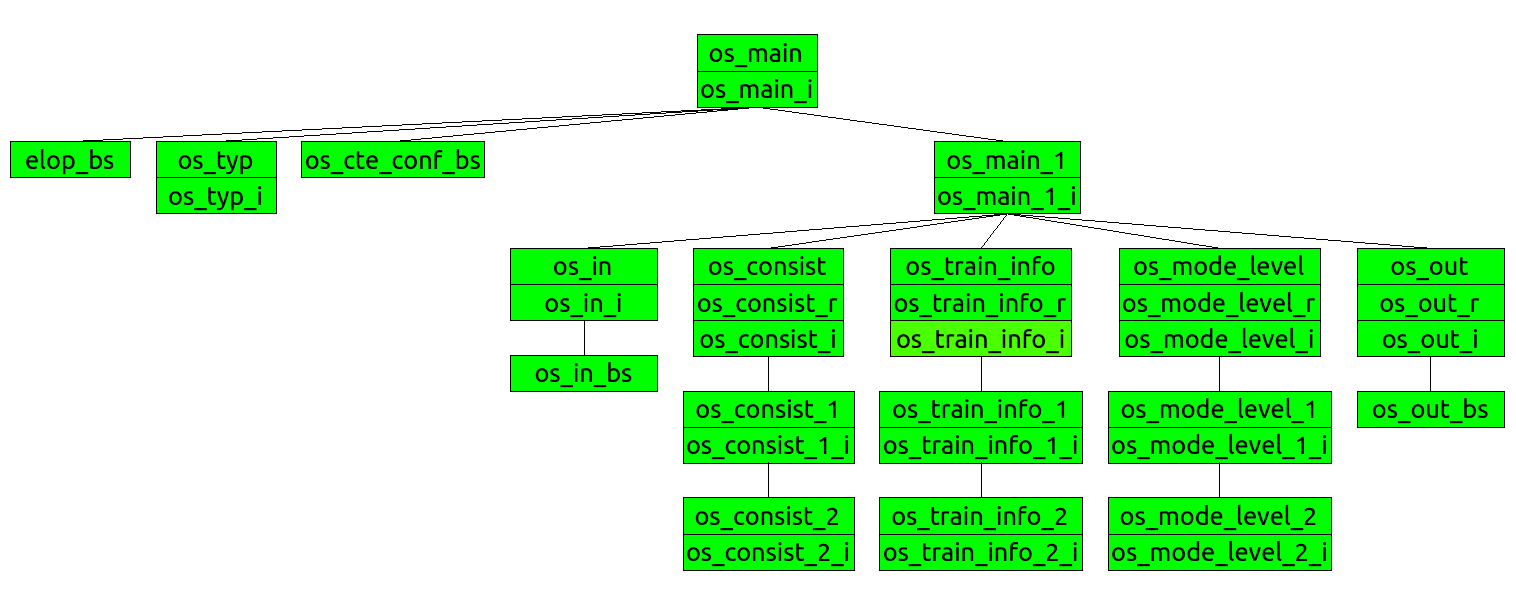
\includegraphics[width=1\textwidth]{procedureos}
\caption{Architecture of the B~model for the Procedure On-Sight example}
\label{fig:procos}
\end{figure}

These three modules are imported by the main sequencer, \verb+os_main_1+, which calls their respective operations. The main sequencer also imports the input module \verb+os_in+, and the output module \verb+os_out+.\\
The typing machine, \verb+os_typ+, and the constant machine, \verb+os_cte_conf_bs+, are both imported by \verb+os_main+, the entry point of the software, which also imports \verb+os_main_1+.\\
 
This ``IMPORTS''-based vertical layout is complemented by a horizontal aspect: the ``SEES'' clause, which enables a component to access another component's data. It is possible for a component to see the components to its left, but not to its right. Thus, a cycle-free graph is maintained.
 
\subsection{Model checking results}
\label{subapp:mc}
ProB has been used on the example model and has shown through model checking that no invariant was violated, and no deadlock state was found. However, for some machines, only a minority of states and nodes have been visited (because of infinite sets in particular) and thus no formal conclusion can be drawn.\\
Additionally, constraint-based checking has also been run and stated, for every operation of every abstract machine, the non-violation of the invariant.

\subsection{Formal proof results}
\label{subapp:proof}
\subsubsection{Project status}
Project status illustrated in figure \ref{fig:atelierb} shows the fully-proved model in Atelier~B.

\begin{figure}[h!]
\centering
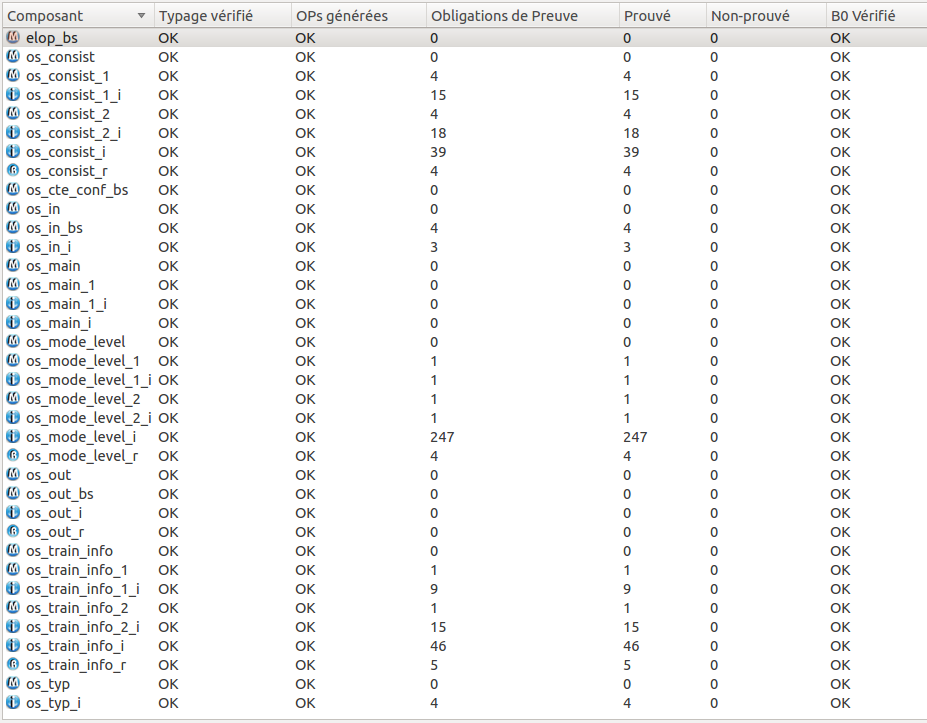
\includegraphics[width=1\textwidth]{atelierb}
\caption{Overview of the B~model in Atelier~B, showing type check, B0 check and proof status}
\label{fig:atelierb}
\end{figure}

This model was proved almost entirely automatically, using the provers with force 0 and force 1. Proving the model results in the certainty of its correctness. In this case, only typing invariants and constraints were expressed, because strong links between the variables do not exist in the example.

\subsubsection{User-defined theories}
When automatic proof fails, the user must provide a manual proof and uses theories for this purpose. Theories are rules that are used to discharge specific goals.\\
In this example, the only module for which interactive proof was required is \verb+os_consist_i+. Below is presented a very simple theory (among several others) used for the proof of this component:

\begin{equation}
\tag{User theory 1}
a < 0 \land 0 \leq b \land 0 < c \Rightarrow a \leq \frac{b}{c}
\end{equation}

This theory is automatically verified by Atelier~B and therefore ensures full consistency of the proof.

\newpage

\begin{thebibliography}{9}
\bibitem{bbook}
	Jean-Raymond Abrial,
	{\itshape The B-Book: Assigning Programs to Meanings},
	Cambridge,
	2005.
\end{thebibliography}

\end{document}



\subsection{Verification and Validation on Event-B models}

The Event-B method share the same language than the classical  B method. Besides both approaches are based on a pre/post -condition mechanism to describe the evolution of the system. Thus similar verification mechanisms can be defined.


\subsubsection{Verification Processes Applicable to Event-B}
\label{sec:verif-proc-appl}

An Event-B model is a formal specification that describes the functional
behavior of a system from a global point of view. In general, an Event-B model
comprises a set of state variables, parametrized events that can modify these
state variables and invariants that describe logical properties thereof.  The
invariants are in first-order predicate logic and can be discharged using
different proof engines, e.g.,\  automatic modern open source SMT solvers and
manual predicate provers.

In general, one starts with a rather abstract description of the model which is
iteratively refined until the desired level of detail is reached. Event-B
supports this refinement by creating the necessary proof obligations that ensure
correct refinement in each step, both for behavioral refinement of events as
well as for data refinement of state variables.

Thanks to the integration into the Eclipse platform, there are many plug-ins
available as extensions. There is a plug-in to use graphical modeling in UML
state machines to describe Event-B models. There is a tight connection to the
ProR requirements engineering plug-in. To facilitate modeling, there are
plug-ins to decompose a model into several sub-models and to facilitate proving
by supporting external formal theories.

Together with the Rodin tool, the Event-B approach was developed in the European
research projects RODIN (2004--2007) and DEPLOY (2008--2012). Since 2011 it is
further developed in the European project ADVANCE\@.

\paragraph{Verification of Type Safety}
\label{sec:verif-type-safety}

Static type checking is a technique that allows the verification of correct
typing for variables at compile / modeling time. It is performed after lexical
and syntactic correctness of the Event-B model have been verified. Static type
checking prevents all type errors at run-time, which eliminates many possible
sources of program errors.

The type system of Event-B is much more expressive than the one of most other
languages, as Event-B also allows the usage of dependent types for variables. In
this case, the type of a variable is dependent of its value, e.g.,\ one can
define the type of all even integers. Event-B can define such types and verify
that events respect the correct dependent typing of variables

In Event-B, every new variable gets a type assigned via a typing invariant. Such
an invariant is either an explicit type assignment or an implicit one, e.g.,\ by
specifying a dependence to another variable which is typed. The integrated type
interference can then deduce the static type of the new variable.

Every event that changes the value of a variable via substitution must also
respect the variable typing. For each event that modifies a variable,  proof
obligations are created that ensure this in a rigorous formal way.

In almost all cases, the proof obligations for type verification are discharged
automatically by the Rodin provers.

\paragraph{Verification of Well-Definedness}
\label{sec:verif-well-defin}

After type checking, one or more well-definedness (WD) proof obligations are
created. This ensures that the expression has a unique meaning and prevents the
usage of expressions that make no sense or are ambiguous.

One prominent example for WD proof obligations in Event-B is the cardinality of
sets. The set of natural numbers $\mathbb{N}$ has countable infinitely many
elements, exactly as many as the set of all even natural numbers
$\mathbb{N}_2:=\{2\cdot n \mid n \in \mathbb{N}\}$. This means that both sets
have the same cardinality, although $\mathbb{N}_2$ is a strict subset of
$\mathbb{N}$.

Therefore, while sets of countable infinite cardinality can be used without any
problem in Event-B models, the usage of cardinality of a set requires the set to
be of finite size which gets verified by an appropriate WD proof obligation.

In almost all cases, the proof obligations for well-definedness are discharged
automatically by the Rodin provers.


\paragraph{Model Simulation}
\label{sec:model-simulation}

A correctly typed Event-B model can be simulated or animated using different
plug-ins like AnimB or ProB. At each step, one of the activated events can be
executed and if applicable parameters for that event can be defined. This allows
for stepping through the formal model, observing the state variables and the
invariants. Using model animation, it is possible to validate the correct
functioning of the model.

\begin{figure}[ht]
  \centering
  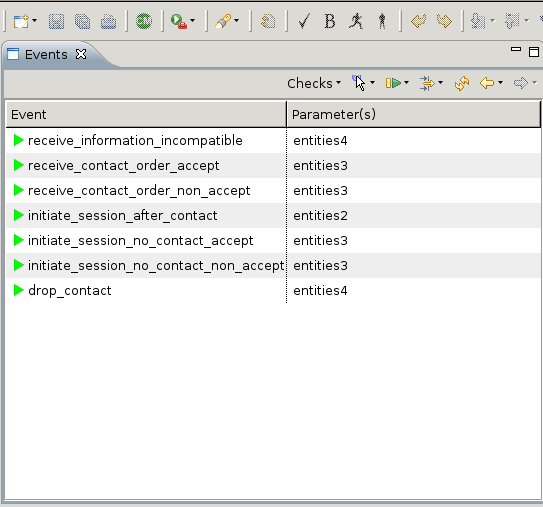
\includegraphics[width=.5\textwidth]{figures/ProBAnimation}
  \caption{ProB Model Animation}
  \label{fig:proBAnimation}
\end{figure}

Figure~\ref{fig:proBAnimation} shows a ProB simulation session. The activated
events are marked green, clicking on them allows for selection of parameters and
to execute the events with the chosen parameters.


\paragraph{Model-Checking of Predicates}
\label{sec:model-check-pred}

Model-checking is a static analysis of the semantics of a model. In general, a
model-checker will create a representation of the whole possible state space of
a model and verify logic properties on this state space. There are many
different possibilities for properties that are verified by model-checkers, some
are listed here:

\begin{itemize}
\item {\bf Equivalence Checking} The equivalence between two models is verified
  given a certain equivalence relation. Often, a specification is compared to
  its (distributed) implementation using bisimulation modulo some reduction
  techniques, e.g.,\ only the externally observable behavior is compared and the
  internal details of the different systems are ignored.
\item {\bf Deadlock Freeness} A deadlock represents a state where the system
  that the system cannot leave as no event is enabled. For a reactive system
  this is always an unwanted state that must be avoided.
\item {\bf Temporal Properties} The evolution of the system over time is
  analyzed, i.e.,\ the admissible event sequences that can lead to different
  states. Roughly, temporal properties comprise \emph{safety properties} which
  describe a set of states that should never be reached and \emph{liveness
    properties} which describe states that should always be reachable. There are
  different temporal logic languages, like LTL and CTL, which allow to describe
  temporal properties of systems.
\end{itemize}

In general, model-checkers suffer from the state space explosion problem. This
means that creating the whole state space becomes often infeasible due to memory
limitations. In general it is also not possible to model-check systems with
infinite state space, like many Event-B models.

In practice, tools like ProB which allow for model-checking of Event-B models,
limit the size of the possible values for variables to a finite subset. While
this means that a correct proof is not possible, it allows for fully automatic
error detection in the model. For any violated property or a deadlock, ProB
provides a counterexample that can be analyzed and therefore allows for
correction of the associated modeling problem.

\begin{figure}[ht]
  \centering
  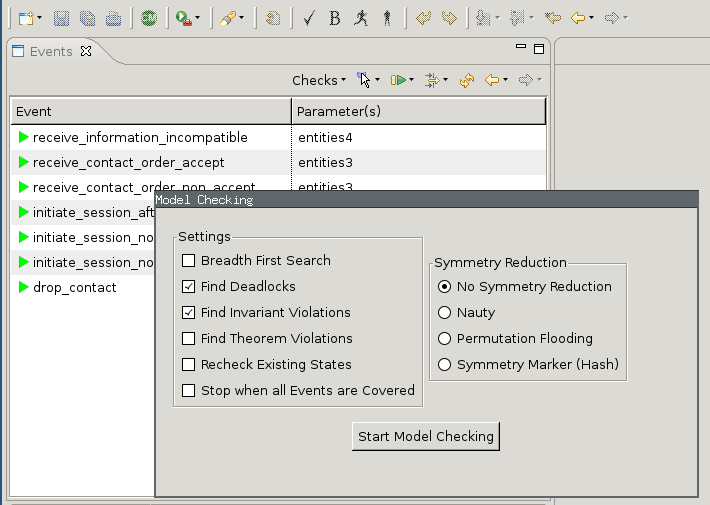
\includegraphics[width=.5\textwidth]{figures/ProBModelChecking}
  \caption{Model-Checking for Deadlocks}
  \label{fig:Prob-model-check}
\end{figure}

Figure~\ref{fig:Prob-model-check} shows the model checking dialog of the Rodin
plug-in for ProB. The currently selected options would check for deadlocks,
i.e.,\ a sequence of events that leads to a situation where no event can be
selected anymore.


\paragraph{Formal Proof of Predicates}
\label{sec:form-proof-pred}

Formal proof techniques provide a much more powerful way to verify predicates
than model-checking. Instead of the creation of the full state-space, they use a
proof calculus to iteratively simplify predicates and to reduce them onto known
lemmas or axioms, thus discharging them.

In contrast to model-checking, formal proof is applicable to models of infinite
size and can cope with undecidable problems. Although this means that there
sometimes will be a manual step in a proof, there are many automated tools that
support formal proofs and can often discharge proof obligations without any
manual intervention.

The Rodin platform natively supports manual construction of formal proofs by
allowing easy access and manipulation of the proof tree and predicate
hypotheses. It also provides access to different automated provers, i.e.,\ the
free of charge AtelierB provers, an open source SMT plug-in that supports
several solvers\footnote{supported open source SMT solvers include: verIT,
  Alt-Ergo, CVC3, Z3} as well as an open source plug-in that connects Rodin to
the Isabelle/HOL proof assistant.

\begin{figure}[ht]
  \centering
  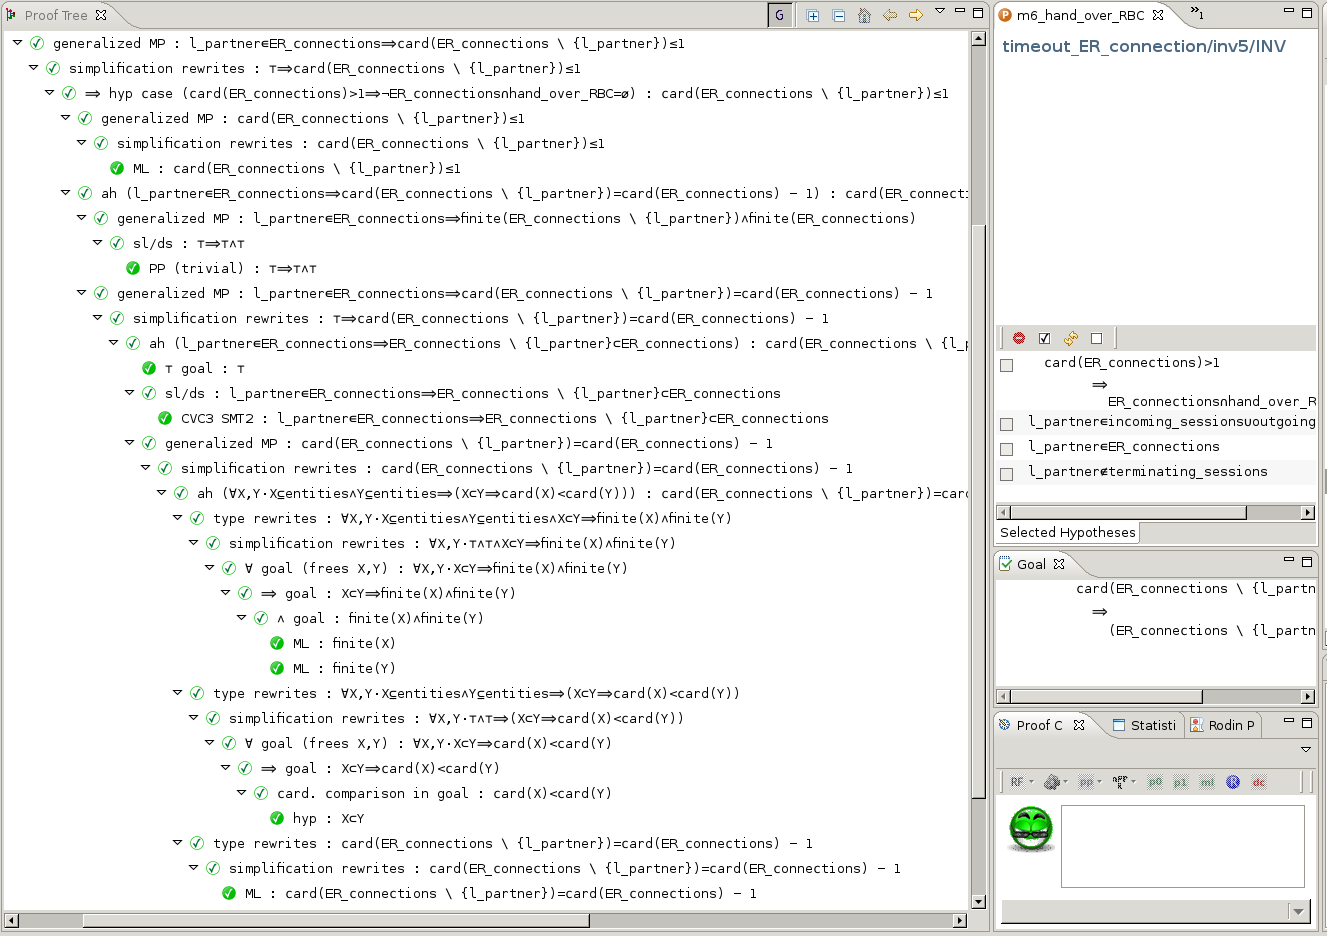
\includegraphics[width=1\textwidth]{figures/ProofTree}
  \caption{Rodin Proof Tree}
  \label{fig:proof-tree}
\end{figure}

Figure~\ref{fig:proof-tree} shows a part of a Rodin proof tree for an
invariant. Its green color signals that the proof is finished, at each node in
the tree, the applied proof rule is shown. This allows for easy inspection of
the proofs and allows both for humans and for machines to verify the correctness
of the proof steps.


\paragraph{Verification of Refinement Correctness}
\label{sec:verif-refin-corr}

Rodin provides extensive support for a top-down development approach and allows
for an iterative refinement of models. The model is developed using different
levels of detail, starting from a rather abstract view, refining the details
where necessary or desired. This refinement process can either be applied to
the events or the variables.

\subparagraph{Data Refinement}
\label{sec:data-refinement}

In general, a data refinement replaces a variable with another one, or multiple
other ones. For example a Boolean variable in the abstract model is replaces by
an enumeration with different possible values. To ensure a correct refinement,
one has to manually supply a ``gluing'' invariant that describes the connection
of the refined and the abstract variable. For example one subset of the possible
values for the enumeration in the refined model would correspond to a value of
``True'' in the abstract model, the remaining values of the enumeration to a
value ``False''. The abstract variable is then deleted from the refined model,
and the necessary proof obligations are created automatically by Rodin.


\subparagraph{Code Refinement}
\label{sec:code-refinement}

For event (or code) refinement, Rodin automatically creates the necessary proof
obligations that ensure that the abstract system is correctly refined by the
more detailed model. This includes the verification that each refining event
only modifies variables that are also modified by the abstract event and that
the modification is equivalent. It also includes verification of guard
strengthening, i.e.,\ the guards of a refining event must be at least as
constraining as of the refined abstract event. A common code refinement is to
split an event in several more specialized ones, where the additional guards
ensure mutual exclusion of the activation conditions.

\begin{figure}[ht]
  \centering
  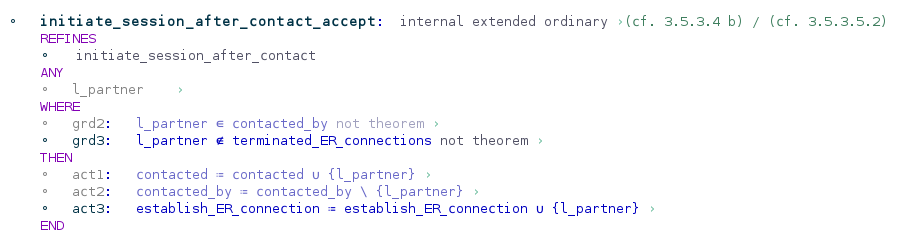
\includegraphics[width=.9\textwidth]{figures/EventRefine}
  \caption{Event Refinement}
  \label{fig:event-refine}
\end{figure}

Figure~\ref{fig:event-refine} shows a refining event with guard strengthening
and an additional variable that is modified. The pale blue colored guards and
actions are derived from the refined event, the darker colored guard and action
are the additional ones for the refining event.


\paragraph{Verification of Design Step Requirements}
\label{sec:verif-design-step}

This section reports on the verification activities of the correct
implementation of the design step requirements. The goal of the activity is to
establish a correct formal representation of the design step requirements.

The activity is described in the Verification and Validation
Plan~\cite{vnvplan}.  In short, it consists of formalizing and proving the
identified requirements of a preceding phase, to ensure their correct
implementation of the requirements. To achieve this, we use the direct
connection of the Event-B model with the ProR based on an EMF model of the
Event-B model.


\paragraph{Verification of Safety Requirements}
\label{sec:verif-safety-requ}

A safety analysis identifies additional requirements which guarantee the safety
of a system. It must be verified that the system model correctly implements
these non-functional requirements. Not every safety requirement is applicable on
the system development level. Many are on the implementation level, e.g.,\ they
demand that certain safety-critical functions are done in a redundant way to
reduce the risk of malfunctioning or loss of that function.

In the safety analysis~\cite{safetyBrice}, a list of safety requirements was
identified using an FMEA analysis of the communication system. A ReqIf file
captures all these safety requirements within ProR, the concerned functional
requirements are traced in the ReqIf file for SS~026 section 3.5.

Each of the safety requirements is examined for applicability in the system
level model, the identified ones are formalized. Most often, the safety
requirements are represented as one or more additional invariants in the system
model. These invariants are linked to the ReqIf file that describes the safety
requirements, ensuring traceability in the model.

\begin{figure}[ht]
  \centering
  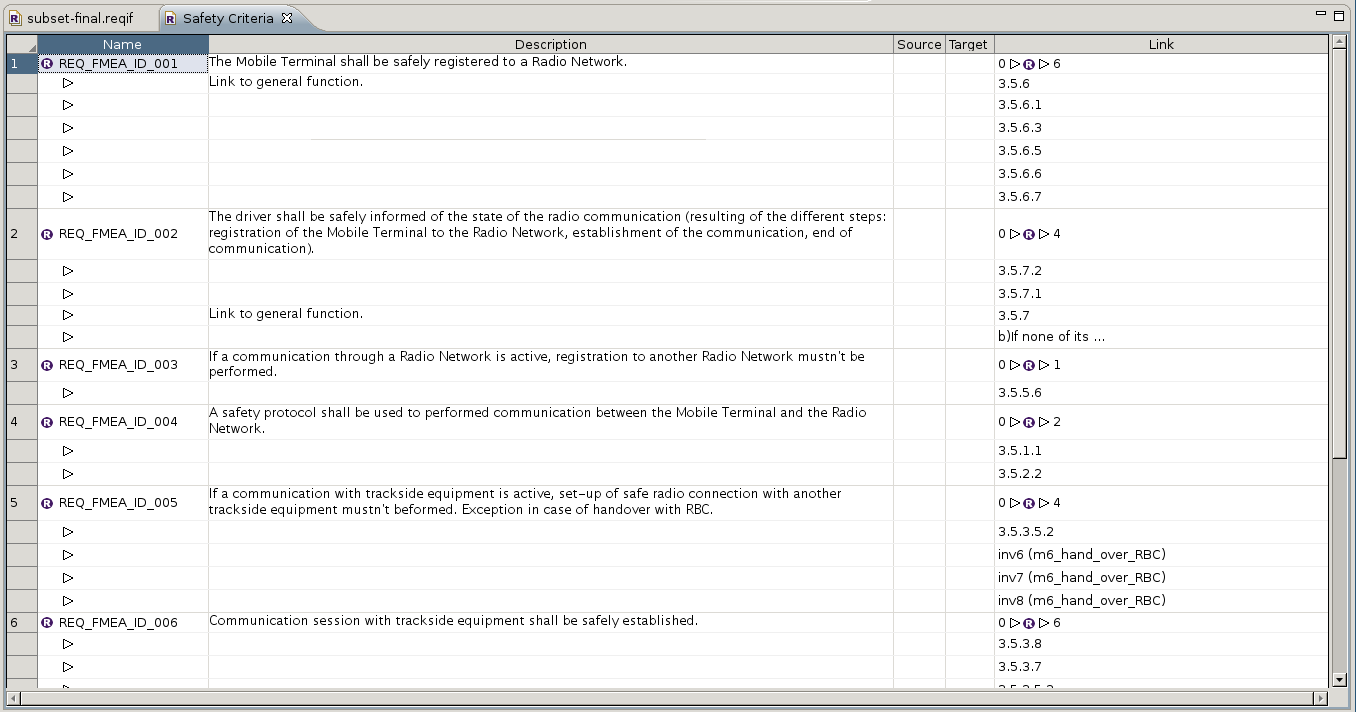
\includegraphics[width=1\textwidth]{figures/ProRSafetyReq}
  \caption{Safety Requirements}
  \label{fig:pror-safety-req}
\end{figure}

Figure~\ref{fig:pror-safety-req} shows a ReqIf document in Rodin (via the ProR
plug-in) which holds the safety requirements defined by the safety analysis. For
each requirement, there are references to the concerned elements of SS~026 and
to Event-B elements where applicable, e.g.,\ {\sf REQ\_FMEA\_ID\_005} which is
linked to the invariants, {\sf inv6}, {\sf inv7} and {\sf inv8}.


\paragraph{Verification of Requirements Coverage}
\label{sec:verif-requ-cover}

This section reports on the verification activities of the coverage of the
design step requirements. The goal of the activity is to establish the coverage
degree of the formal representation of the design step requirements.

The activity is described in the Verification and Validation
Plan~\cite{vnvplan}.  In short, in consists of analyzing the coverage of the
identified requirements of a preceding phase, to ensure their completeness of
implementation of the requirements wrt.\ the refinement level of the model. To
achieve this, we use the direct connection of the Event-B model with the ProR
based on an EMF model of the Event-B model.


\subsubsection{Object of Verification}
\label{sec:object-verification}

The object of verification is the Event-B model for the communication
establishing\footnote{\url{https://github.com/openETCS/model-evaluation/tree/master/model/Event_B_Systerel/Subset_026_comm_session}}. It
is from the strictly formal modeling phase and represents the communication
session management of the OBU\@.

\paragraph{Available Specification}
\label{sec:avail-spec}

The model implements the requirements for the communication session management
as described in SS~026, section 3.5\cite{subset-26}.

This section describes the establishing, maintaining and termination of a
communication session of the OBU with on-track systems.

%\subsubsection{Detailed verification plan}
%\label{sec:deta-verif-plan}

\paragraph{Goals}

One goal is the development of a strictly formal, fully proven model of the
communication session management and to provide evidence of covering the
necessary requirements of SS~026 as well as proving correctness of the model
wrt.\ the requirements ans attaining a good coverage of the model wrt.\ the
requirements.

The second goal is to correctly implement the applicable safety requirements
identified by the safety analysis. Both functional and safety requirements
should be traced in the model and a requirement document in a standardized
format.

The formal model will represent the described functionality on the system level,
the correct functioning can be validated by step-wise simulation and
model-checking of deadlock-freeness.


\paragraph{Method/Approach}
\label{sec:methodapproach}

At first, the basic functionality described in the section 3.5 that are
identified. These serve as basis for a first abstract model, which is refined
iteratively, adding the desired level of detail. The elements of SS~026 are
traced using links from Event-B to the ProR file in ReqIf format. Requirements
are formalized as invariants and proven where applicable.

\paragraph{Means}
\label{sec:means}

The means used are:
\begin{itemize}
\item open source Rodin tool (\url{http://www.event-b.org/}), including plug-ins
  (for details
  see~\url{https://github.com/openETCS/model-evaluation/blob/master/model/Event_B_Systerel/Subset_026_comm_session/latex/subset_3_5.pdf})
\item ProR requirements modeling tool~\url{http://www.pror.org}
\item open source ProB model checker and B model
  simulator~\url{http://www.stups.uni-duesseldorf.de/ProB/index.php5/Main_Page}
\item open source CVC3 (\url{http://www.cs.nyu.edu/acsys/cvc3/}), verIT
  (\url{www.verit-solver.org}) and Alt-Ergo (\url{http://alt-ergo.lri.fr}) SMT
  solvers
\end{itemize}

% \subparagraph{Other}

%  \bgcmmnt{optional, might be renamed}

\paragraph{Results}
\label{sec:results}

\begin{itemize}
\item The result is a fully formal model of the communication session management
  as described in section 3.5 of SS~026.
\item Each implemented element of this section is linked to the ProR
  requirements file, both specification elements that describe how something has
  to be done, as well as requirements that describe what must be achieved.
\item The model can be simulated / animated, either with the AnimB or the ProB
  plug-in, validating the functional capabilities.
\item The requirements are formalized as invariants in predicate logic, their
  proofs are for the most part fully automatic.
\item It was found that while the SS~026 communication management explicitly
  allows multiple communication partners (see RBC handover), there is no
  explicit limit of established communication connections given in section 3.5.
\item A complete covering of the elements of SS~026 was not realized, e.g.,\
  there is a representation of the contents of a message, but its explicit
  format is not implemented. This is considered an implementation detail without
  influence for a system level analysis. In general, Event-B models will not be
  refined up to the implementation level.
\end{itemize}

\paragraph{Summary}

The created fully formal functional model allows for formalization and proof of
SS~026 requirements. The integration of Rodin into Eclipse provides easy access
to extensions like the ProR requirements tool which allows for validation of
coverage of requirements.

The integration of various provers, in particular the SMT plug-in automates a
large part of the formal verification. For the model of the communication
management, from 382 non-trivial\footnote{many WD proof obligations are so
  trivial that they will not be shown in Rodin} proof obligations, only 12,
i.e.,\ $3.2\%$ require any manual intervention.

\paragraph{Evidence produced}
\label{sec:evidence-produced}

The formal Event-B model, including a ReqIf document for section 3.5 of SS~026
and a pdf documentation of the model can be found at
\url{https://github.com/openETCS/model-evaluation/tree/master/model/Event_B_Systerel/Subset_026_comm_session}

\subsubsection{Conclusions/Lessons learned}

Having an abstract formal model of the implemented functionality which can be
simulated, allows for interesting insights into the overall functioning of a
system. Formalized requirements are very helpful in both the identification of
ambiguous requirements and in their clarification.

The elements of SS~026 are of very different nature. Some describe rather
low-level specification details, other describe ``real'' requirements. Without
an analysis as done with this Event-B model, it can be difficult to decide which
elements must be considered on a system level analysis and which on the lower
implementation level.


\subsubsection{Future Activities}
\label{sec:future-activities}

For other sections of SS~026, that describe a functionality in a way that can be
captured in an iteratively refined model and which has interesting requirements
on a rather high level, creating an Event-B model can provide insight into the
functioning, identify ambiguous or erroneous elements in the specification and
can provide the basis for logical pre- and post conditions of the later
implementation.



\subsection{Verification processes applicable to a\\SCADE~model}

The verifier shall be independent and shall neither be Requirements Manager, Designer nor Implementer as defined in the safety standards EN 50128 v2011.

The input documents needed are all the necessary System and Software Documentation used for the SCADE design activity and all the documentation produced during this phase, such as the SCADE Design Description, the SCADE Design Test Specification and the SCADE Design Test Report.

\subsubsection{Respect of modelling rules}

Syntactic rules of SCADE language are verified with the Quick Check tool available in the publisher. If an error is detected it must be corrected or justified in the SCADE Design Description document by the designer. The verifier shall ensure that no error remains or the justification associated is correct.

For specific modelling rules the verification has to be made manually by the verifier and described in the Verification Report. A grid of verification may be created in order to prove the compliance of the model with the rules. On some cases, dedicated tools can be developed.

\subsubsection{Specification traceability check}

The verification of the compliance of the SCADE model with each requirement has to be made manually, by the verifier. 

The Scade model shall be correct according to the informal requirements and the informal specification shall be completely covered : each specification requirement must be traced in the SCADE model. The specification requirements which are not covered by the SCADE model must be listed and justified in the SCADE Design Description document by the designer.

\subsubsection{Testing and Validation of the model}

The verifier shall control the activity of software testing performed by the tester.

The software testing uses the Model Test Coverage (MTC) and the Generic Qualified Testing Environment (QTE) tools from SCADE. Five steps are performed.
\begin{itemize}
\item Establish the Test Specification document.
\item Writing scenarios in order to test the different functions independently.
\item Running scenarios on the SCADE model.
\item Extraction and analysis of results and the associated coverage.
\item Establish the Test Report.
\end{itemize}

\subsection{Results}

All these different verifications activities shall be described in the Verification and Validation Plan, and their results shall be record in a Verification Report. Each disparity must be corrected or justified.

\subsubsection{Verification report content}

The verifier shall produce a Verification Report containing the proof of the compliance of the SCADE model. It shall include the following points:
\begin{itemize}
\item the identity, version and configuration of SCADE model;
\item the verifier name;
\item the goal of the Verification Report;
\item the result of each verification process with:
\subitem - items which do not conform to the specifications;
\subitem - components, data, structures and algorithms poorly adapted to the problem;
\subitem - detected errors or deficiencies.
\item the fulfilment of, or deviation from, the Software Verification Plan;
\item assumptions if any;
\item a summary of the verification results.
\end{itemize}

\subsection{Conclusion}

The use of SCADE with its verification processes is compliant with the CENELEC norm but as it is not developed as open-source it is not compliant with the goal of openETCs project. 


\newpage

\newcommand{\uml}{UML\xspace}
\newcommand{\marte}{MARTE\xspace}
\newcommand{\tpn}{TPN\xspace}
\newcommand{\sysml}{SysML\xspace}

\section{LAAS and INPT: Verification of the  Ceiling Speed Monitoring}
\label{sec:laas}
This section reports the verification activity of the Ceiling Speed Monitoring (CSM) function provided by the University of Bremen using the Tina model-checking toolbox {http://projects.laas.fr/tina/}. The goal of this activity is to use an automatic transformation from SysML to Time Petri Net (TPN) to this model and check several temporal logic formulas on the resulting system.  

\subsection{Object of verification}

We study the SysML model of CSM function using the Tina model-checking toolbox. 
We base our analysis on a model provided by the University of Bremen that was slightly
extended with information on the environment of the system. The same
function was studied by the University of Rostock using a software
testing approach.

The cornerstone of our approach is an automatic transformation from
SysML models to TPN models. We can then use the resulting formal
model to check several temporal logic formulas.

\subsection{Available specification}

The CSM function supervises the observance of the maximal speed allowed according to the current most restrictive speed profile (MRSP). The model was edited, and later extended, using Papyrus. 
The specification of the system under test is described in \cite{csmwp4} and available here: \url{https://github.com/openETCS/validation/tree/master/VnVUserStories/VnVUserStoryUniBremen}.  

To provide executable models for the CSM function, an environment model needs to be defined; mainly the possible actions on the current speed of the train resulting from 
acceleration or deceleration orders. 

The combination of a test environment model and an optional test driver
model provides a deterministic model. 

\subsubsection{Description of the Environment Model}
The environment model is defined in the TestEnvironment block. It is
described using a state machine diagram as shown in
Figure \ref{fig:env}.

\begin{figure}[ht!]
	\centering
	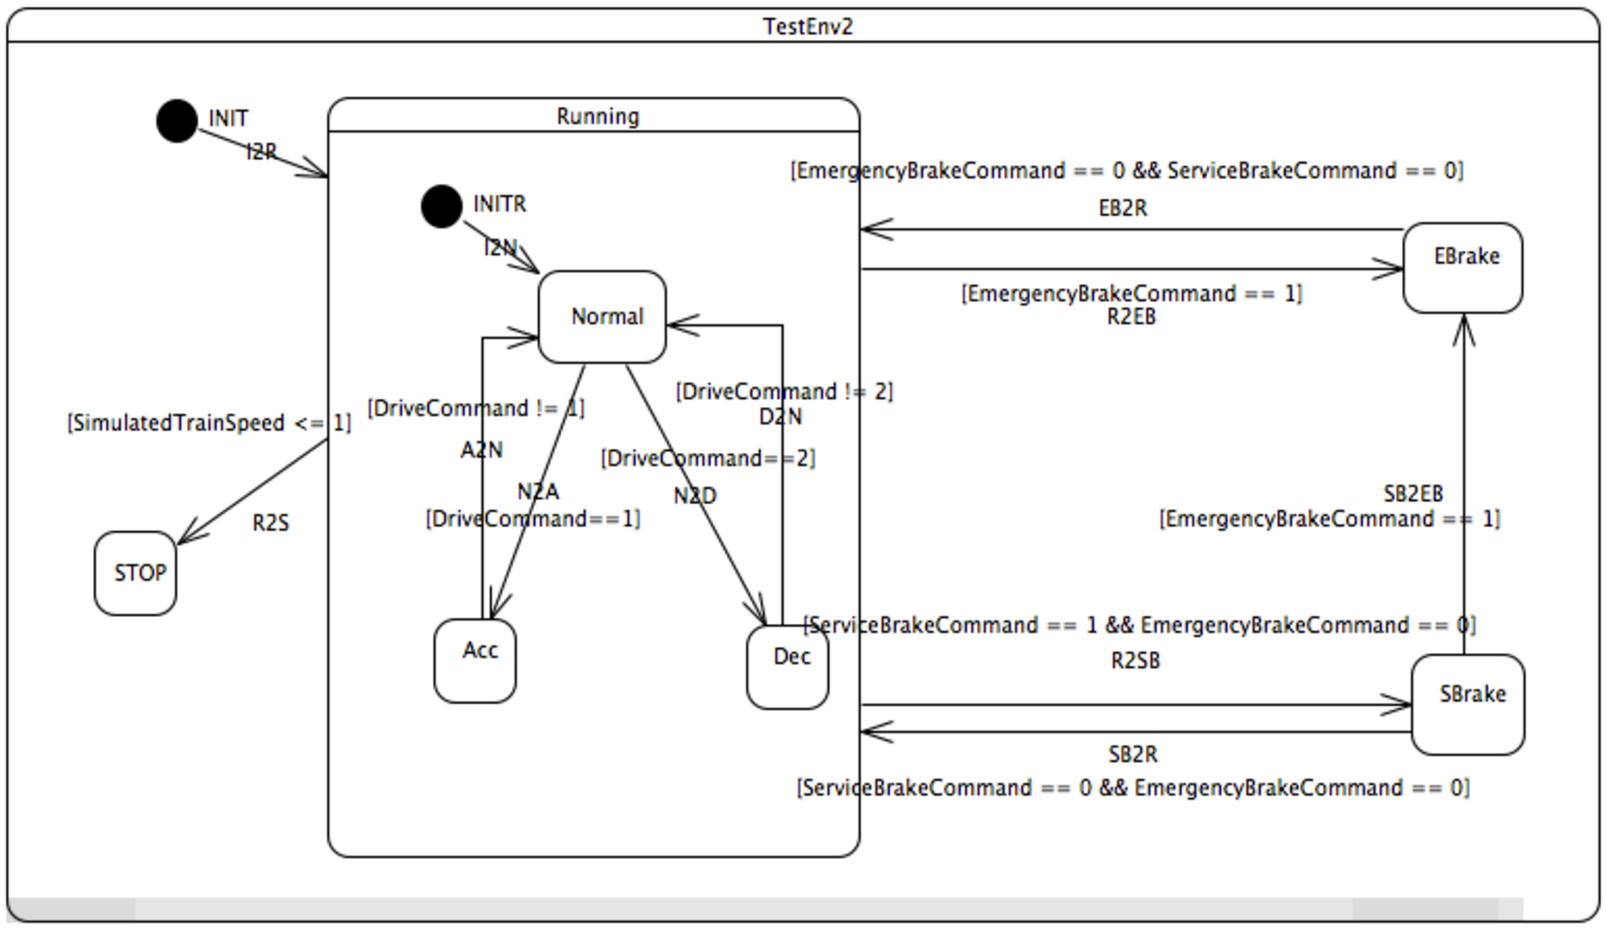
\includegraphics[height=0.34\textheight]{figures/env}
	\caption{CSM Test Environment Model}
    \label{fig:env}
\end{figure}

The system under test is activated with an initial speed
(SimulatedTrainSpeed) and may enter into the composite state Running.
The Running state encapsulates three possible behavior. Either the
speed remains unchanged (state Normal), or the train accelerates
(state Acc), or the train decelerates (state Dec). The guards defined
on the transitions found inside the composite state Running are
described in Table \ref{tab:runningtr}. The DriveCommand is the
command sent by the driver which contains three modes: keeping speed
(DriveCommand = 0), acceleration (DriveCommand = 1) and Deceleration
(DriveCommand = 2).

\begin{table}[ht!]
\footnotesize
	\caption{Transitions between Running States}
	\begin{center}
    \begin{tabular}{|c|c|c|c|}
    \hline
    To $\setminus$ From  & Normal & Acc & Dec \\
    \hline
    Normal &   &  DriveCommand != 1  & DriveCommand != 2\\
    \hline
    Acc  & DriveCommand == 1 & &  \\
    \hline
    Dec  & DriveCommand == 2 & & \\
	\hline
    \end{tabular}
    \end{center}
\label{tab:runningtr}
\end{table} 

The actions on each transition (the "do behaviors") are described in
Table \ref{tab:runningdo}. At the moment we use dummy values for the
acceleration and braking parameters of the train. We have chosen a fix
acceleration of 2 km/h per 100 units of time (t.u.) and a constant
braking factor of 2 km/h per 400 t.u.

\begin{table}[ht!]
\footnotesize
	\caption{Do Behaviors in Running States}
	\begin{center}
    \begin{tabular}{|c|c|}
	\hline    
    Normal & \\
	\hline    
    Acc & SimulatedTrainSpeed = SimulatedTrainSpeed + 2; \\
	\hline    
    Dec & SimulatedTrainSpeed = SimulatedTrainSpeed - 2;\\
	\hline
    \end{tabular}
    \end{center}
\label{tab:runningdo}
\end{table} 

The effect of the environment on the system is described by the
transitions between states Running, EBrake (emergency brake), SBrake
(service brake) and STOP (simulatedTrain Speed <= 1). The transition
guards between environment states are described in Table
\ref{tab:envtr}. The transitions are controlled by the commands
EmergencyBrakeCommand and ServiceBrakeCommand generated from the train
control system.

\begin{table}[ht!]
\scriptsize
	\caption{Transitions between Environment States}
	\begin{center}
    \begin{tabular}{|c|c|c|c|c|}
    \hline
    To $\setminus$ From  & Running & EBrake & SBrake & STOP \\
	\hline
	Running & & \begin{tabular}[x]{@{}c@{}}ServiceBrakeCommand == 0 \&\& \\ EmergencyBrakeCommand == 0\end{tabular}  &\begin{tabular}[x]{@{}c@{}}ServiceBrakeCommand == 0 \&\& \\ EmergencyBrakeCommand == 0\end{tabular}     & \\
	\hline
	EBrake &  EmergencyBrakeCommand == 1  & &\begin{tabular}[x]{@{}c@{}}ServiceBrakeCommand == 0 \&\& \\ EmergencyBrakeCommand == 1\end{tabular} & \\
	\hline
	SBrake &  \begin{tabular}[x]{@{}c@{}}ServiceBrakeCommand == 1 \&\& \\ EmergencyBrakeCommand == 0\end{tabular}  & \begin{tabular}[x]{@{}c@{}}ServiceBrakeCommand == 1 \&\& \\ EmergencyBrakeCommand == 0\end{tabular}   & & \\
	\hline
	STOP &  SimulatedTrainSpeed <= 1 & & & \\
	\hline
    \end{tabular}
    \end{center}
\label{tab:envtr}
\end{table} 

The do behaviors in environment states are described in Table
\ref{tab:envdo}. The deceleration of emergency brake is set at 10 km/h
per 200 t.u.. The deceleration of service brake is set at 5 km/h per
200 t.u..

\begin{table}[ht!]
  \footnotesize
  \caption{Do Behaviors in Environment States}
  \begin{center}
    \begin{tabular}{|c|c|}
      \hline    
      Running & \\
      \hline    
      EBrake & SimulatedTrainSpeed = SimulatedTrainSpeed - 10; \\
      \hline    
      SBrake & SimulatedTrainSpeed = SimulatedTrainSpeed - 5;\\
      \hline
      STOP & \\
      \hline
    \end{tabular}
  \end{center}
  \label{tab:envdo}
\end{table} 

\subsubsection{Description of the Driver Model}

In addition to the model of the train behavior we have added a model
of the driver (and of the track description) that can be used to force
a particular scenario. In this context, a scenario is a timed
annotated sequence of acceleration and deceleration orders. One
possible scenario can be obtained using the model defined in the
TestDriver block of Fig. \ref{fig:driver}. This test describes a
situation where the driver accelerates for a time T1 (DriveCommand =
1) before decelerating for a time T2. 

\begin{figure}[ht!]
  \centering
  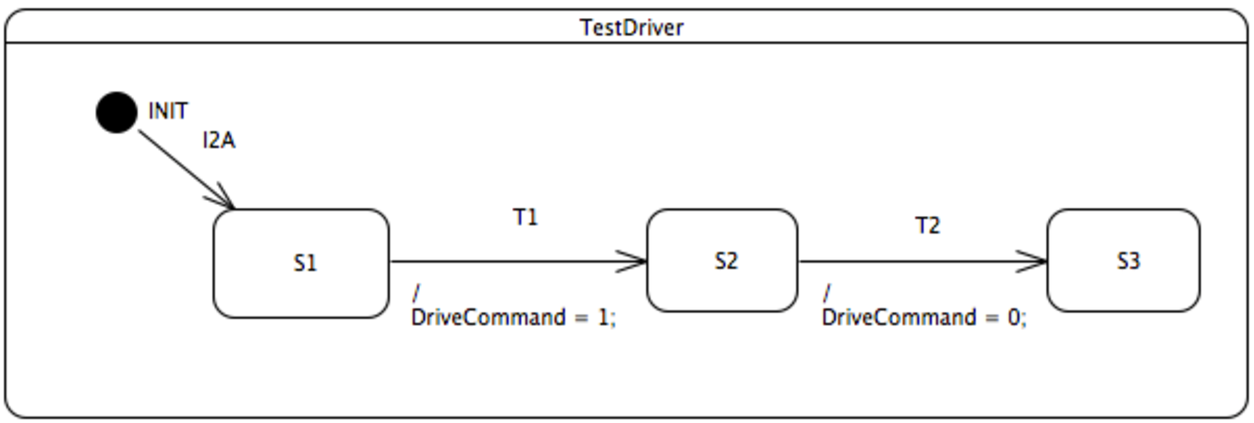
\includegraphics[height=0.18\textheight]{figures/driver}
  \caption{Test Driver Model}
  \label{fig:driver}
\end{figure}

\subsection{Detailed verification plan}

\subsubsection{Goals}

Our main goal is to reuse the existing CSM model and extend the environment model with the driver model. These SysML models are then transformed to TPN models to validate the specification by model-checking. 

\subsubsection{Method/Approach}

We first provide some background information on the transformation from
SysML to TPN used in our study. This transformation
is based on a mapping from UML (Unified Modeling Language) to TPN
described in the PhD thesis of Ning Ge~\cite{Ge2014}. The
transformation can also take into account real-time properties defined
using the MARTE profile (Modeling and Analysis of Real Time and
Embedded systems). 

By nature, UML is intended to be a general purpose modeling language
and, as such, it integrates different modeling viewpoints through the
definition of a large class of diagram elements. In the work of Ge, they
select a core subset of UML diagrams and diagram elements for
modeling real-time software architecture and behavior, and focus on
the semantic mapping from the UML model to the verification model.

We briefly describe the different elements supported in our
translation.

\textbf{Architecture Model}
The purpose of architecture model is to connect different sub-system
behavior models and create a system-level model, by means of
communication media. The objective of the mapping is to replace each
architecture model's entities by its relevant behavior model.  We rely
on the composite structure diagram as the architecture model.
Composite structure diagrams specify the internal structure of a
class, including its interaction points to other parts of the system,
and the architecture of all parts managed by this class. They are used
to explore run-time instances of interconnected instances
collaborating over communications links.

\textbf{Behavioral Model}
The mapping semantics for behavioral model covers both activity and
state machine diagrams.

Activity diagrams express the coordination between lower-level
behaviors using constraints on the possible sequence of actions. In
this context, actions can be triggered because other actions finish
executing; because objects and resources become available; or because
external events occur. The main elements in \uml activity diagram
behavior model are control nodes, actions, objects, and connection
elements.


\textbf{Principles of Semantic Mapping}

The mapping from \uml-\marte to TPN preserves the semantics of the
input language. A particularity of the approach is that, for
efficiency reason, the transformation is driven by the set of
real-time properties that should be checked on the resulting
model. For instance, in order to reduce the size of the state space
explored during the verification phase, the behavior of some elements
irrelevant to the target property can be abstracted. The
transformation conforms to the following principles:
%%
\begin{itemize}
\item The resulting \tpn models should be easy to analyze, meaning
  that the semantics mapping should allow the use of high-level
  abstraction methods during model-checking.
\item In order to keep the transformation simple, we use a
  compositional approach where the resulting system is obtained by
  composing the interpretation of all its elements. Then, to optimize
  the result, we apply a state space reduction phase that eliminates
  the elements irrelevant to the verification.
\end{itemize}


\subsubsection{Means}
Instead of the thirteen diagrams available in \uml 2, the \sysml
includes only nine diagrams, including:
%%
\begin{itemize}
\item
the Block Definition Diagram (BDD), replacing the \uml 2 class diagram
\item
the Internal Block Definition Diagram (IBDD), replacing the \uml 2 composite structure diagram
\item
the Parameter diagram, a \sysml extension to analyze critical system parameters
\item
the Package diagram remained unchanged. 
\end{itemize}

The behavior diagrams includes:
\begin{itemize}
\item
the activity diagram, slightly modified from \uml 2
\item
the sequence, state machine, and use case diagrams remain unchanged. 
\end{itemize}

The requirement diagram is a \sysml extension to describe functional, performance, and interface requirements.	

In order to reuse the existing transformation form \uml to
TPN~\cite{Ge2014} to build a mapping from SysML, we have redefined the
mapping semantics for the block diagram as structure models. The
mapping semantics for the activity and state machine diagrams are left
unchanged. Some of the semantics mapping have also been modified in
order to take into account some of the modeling convention adopted in
the OpenETCS project.

Also, the target model is now an extension of  TPN with
priorities and typed variables called TTS, for Time Transition
System. The data handling ability of TTS is used to model the guards
and actions on integer and float variables found in a SysML diagram.


\subsection{Results}

We provide two verification scenarios for testing the formal system
obtained from the transformation of the CSM model. Each scenario is
available as a TTS "file" (actually a folder called tpn.tts) inside
the 05-Work folder.

\textbf{Scenario 1}
Scenario 1 includes the following initial values for the parameters:
\begin{itemize}
\item
SimulatedTrainSpeed = 110
\item
V\_mrsp = 120
\item
SBAvailable = true
\item
DriveCommand = 1. The initial drive command is acceleration. 
\item
T1 transition in Driver model has an effect behavior DriveCommand = 1. The time duration for the initial behavior (acceleration) is 20000. 
\item
T2 transition in Driver model has an effect behavior DriveCommand = 0. The time duration for the behavior before keeping speed (acceleration) is 10000. 
\end{itemize}

We give in the table below the number of reachable states (or
markings) of the resulting TPN. A marking is defined by a particular
value for each system variable and for each internal state of the
blocks. This gives a rough idea of the complexity of checking
reachability properties on the system. "Classes" take into account
timing constraints on top of the markings; hence there is always more
classes than markings. The generation of the whole state space takes
for Scenario 1 takes
less than 24 seconds (system time: 23.350s).\\

\begin{table}[ht!]
\footnotesize
\caption{State Space of Scenario 1}
\begin{center}
  \begin{tabular}{|c|c|c|c|}
    \hline
    markings & domains & classes & transitions \\
    \hline
    399 & 455880 & 456926 & 978970 \\ 
    \hline
  \end{tabular}
\end{center}
\end{table}

\textbf{Scenario 2}
Scenario 2 includes the following initial values of parameters:
\begin{itemize}
\item
SimulatedTrainSpeed = 0
\item
V\_mrsp = 160
\item
SBAvailable = true
\item
DriveCommand = 1. The initial drive command is acceleration. 
\item
T1 transition in Driver model has an effect behavior DriveCommand = 2. The time duration for initial behavior (acceleration) is 200000. 
\item
T2 transition in Driver model has an effect behavior DriveCommand = 0. The time duration for the behavior before keeping speed (deceleration) is 100000. 
\end{itemize}

The size of the state graph for scenario 2 is shown in the table
below. The generation of the whole state space takes less than 26s
(system time of 25.912s).


\begin{table}[ht!]
\caption{State Space of Scenario 2}
\footnotesize
\begin{center}
  \begin{tabular}{|c|c|c|c|}
    \hline
    markings & domains & classes & transitions \\
    \hline
    474 & 700129	 & 700472 & 1201679 \\ 
    \hline
  \end{tabular}
\end{center}
\end{table}

\textbf{Verification of Requirements} 
We have used our model-checking toolbox to check the properties stated
in the work by Univ. Bremen~\cite{csmwp4}. These properties are a
direct translation into temporal logic of the requirements found on
the Subset-026. Since the CSM model does not take into
account the possible activation and de-activation of the CSM, we have
not dealt with three requirements. (By default, the CSM is always
activated.) We provide an interpretation of the nine remaining
requirements using LTL, see Table \ref{tab:reqltl}. To simplify the
the LTL formula, we have used simple names for naming the relevant
variables. Full names, integrating information on the hierarchy,
should be used when model-checking the actual systems in Tina.


\begin{table}[ht!]
\footnotesize
	\caption{LTL}
	\begin{center}
    \begin{tabular}{|c|p{10cm}|}
    \hline
	Requirement & LTL Formula \\
	\hline
	\hline
	req\_01 & EmergencyBrakeCommand $\wedge$ SBAvailable=0 $\wedge$ SimulatedTrainSpeed <= V\_mrsp $\wedge$  RevocationEmergencyBrake=0\\
	\hline
	req\_02 & ServiceBrakeCommand $\wedge$ SBAvailable=0 $\wedge$ SimulatedTrainSpeed <= V\_mrsp\\
	\hline
	req\_03 & ServiceBrakeCommand $\wedge$ SBAvailable=0 $\wedge$ SimulatedTrainSpeed gt (V\_mrsp + dV\_sbi) $\wedge$ SimulatedTrainSpeed lt (V\_mrsp + dV\_ebi) \\
	\hline
	req\_08 &  $\diamond$ ((NORMAL	 $\wedge$ SimulatedTrainSpeed <= V\_mrsp) U (NORMAL $\wedge$ SimulatedTrainSpeed gt V\_mrsp + dV\_warning $\wedge$ SimulatedTrainSpeed <= V\_mrsp + dV\_sbi)) \\
	\hline
	req\_09 & $\diamond$ ((NORMAL $\wedge$ SimulatedTrainSpeed <= V\_mrsp) $\wedge$ ((NORMAL $\wedge$ SimulatedTrainSpeed <= V\_mrsp) U (NORMAL $\wedge$ SimulatedTrainSpeed gt V\_mrsp + dV\_sbi $\wedge$ SimulatedTrainSpeed <= V\_mrsp + dV\_ebi))) \\
	\hline
	req\_10 & $\diamond$ ((NORMAL $\wedge$ SimulatedTrainSpeed <= V\_mrsp) $\wedge$ ((NORMAL $\wedge$ SimulatedTrainSpeed <= V\_mrsp) U (NORMAL $\wedge$ SimulatedTrainSpeed gt V\_mrsp + dV\_sbi)))\\
	\hline
	req\_11 & $\diamond$ ((OVERSPEED $\wedge$ SimulatedTrainSpeed <= V\_mrsp) $\wedge$ ((OVERSPEED $\wedge$ SimulatedTrainSpeed <= V\_mrsp) U (NORMAL $\wedge$ SimulatedTrainSpeed gt V\_mrsp + dV\_sbi $\wedge$ SimulatedTrainSpeed <= V\_mrsp + dV\_ebi))) \\
	\hline
	req\_12 & $\diamond$ ((OVERSPEED $\wedge$ SimulatedTrainSpeed <= V\_mrsp) $\wedge$ ((OVERSPEED $\wedge$ SimulatedTrainSpeed <= V\_mrsp) U (NORMAL $\wedge$ SimulatedTrainSpeed gt V\_mrsp + dV\_sbi))) \\
	\hline
	req\_13 & $\diamond$ ((WARNING $\wedge$ SimulatedTrainSpeed <= V\_mrsp) $\wedge$ ((WARNING $\wedge$ SimulatedTrainSpeed <= V\_mrsp) U (WARNING $\wedge$ SimulatedTrainSpeed gt V\_mrsp + dV\_ebi))) \\
	\hline
    \end{tabular}
    \end{center}
\label{tab:reqltl}
\end{table} 


\subsection{Summary}

What we have done:
\begin{enumerate}
\item Extended an environment model and a driver model in SysML for the CSM function.
\item Transformed SysML models to TPN models.
\item Verified LTL properties using Tina model-checking toolset on the TPN models.
\end{enumerate}

\subsection{Conclusions/Lessons learned}

To provide deterministic verification scenarios, we have extended the CSM models defined by Uni Bermen with an environment model and a driver model. 
The transformation from semi-formal SysML model (including block, activity and state machine diagrams) to the TPN model is automatic. The resulting TPN models are then used to validate system specification written by LTL. 

For now, there is still no state space explosion problem in this case study. We intend to verify the Speed and Distance Monitoring function model to further evaluate our method. 

\subsection{Future Activities}
 \begin{enumerate}
 \item Refine the environment model by describing desired test scenarios using the test scenarios defined by Uni Bremen. 
 \item Model and verify the calculation of train position either by using the existing SCADE model or by refining the SysML model.
 \item Encapsulate the transformation tool as an independent eclipse plugin. 
 \end{enumerate}

%\bibliographystyle{plain}
%\bibliography{biblio}



\section{Conclusion}

This Deliverable presented the formal \vv of Institut
Mines-Telecom, TWT GmbH Science \& Inovation, University of Bremen, University of Rostock, Systerel, LAAS-CNRS and INPT. 
The V\&V activities are focused on the System Requirement Specifications in
Subset-026 such as the Movement Authority (chap. 3.8), the Procedures (chap. 5),
the Management of the Radio Communication (chap. 3.5), the Speed and Distance
Monitoring (chap. 3.13), the Procedure on-Signt (chap. 5), and the Ceiling Speed Monitoring (part of the Speed and Distance Monitoring). 

These SRSs have been formalized in formal models such as  Extended Timed Finite
State Machine, Colored Petri-Net, SCADE, Classical B, Event B and Time Petri Net. 
The V\&V have been done on these models. They resulted
the correctness of the SRS but also
some inconsistencies, ambiguities and gaps in SRS being
repported in the Specification Findings.

The next steps are to refine the formal models and then to do the V\&V.
The specification findings will be updated during this process.
The test generation and then execution against the
simulators will be also focused.




%\nocite{*}
%===================================================
%Do NOT change anything below this line

%\bibliographystyle{IEEEtran}
\bibliographystyle{unsrt}

\bibliography{biblio}
%

\end{document}
